\def\DTExplainerLanguage{vi}
\documentclass[11pt,a4paper]{article}
% Shared visual and semantic style for the D-Tracker explainers.
\NeedsTeXFormat{LaTeX2e}
\RequirePackage{etoolbox}
\providecommand{\DTExplainerLanguage}{en}

\ifdefstring{\DTExplainerLanguage}{vi}{%
  \RequirePackage[main=vietnamese,english]{babel}%
}{%
  \RequirePackage[main=english]{babel}%
}

\RequirePackage{fontspec}
\setmainfont{TeXGyrePagellaX-Regular.otf}[
  BoldFont=TeXGyrePagellaX-Bold.otf,
  ItalicFont=TeXGyrePagellaX-Italic.otf,
  BoldItalicFont=TeXGyrePagellaX-BoldItalic.otf
]
\setsansfont{texgyreheros-regular.otf}[
  BoldFont=texgyreheros-bold.otf,
  ItalicFont=texgyreheros-italic.otf,
  BoldItalicFont=texgyreheros-bolditalic.otf
]
\setmonofont{texgyrecursor-regular.otf}[
  BoldFont=texgyrecursor-bold.otf,
  ItalicFont=texgyrecursor-italic.otf,
  BoldItalicFont=texgyrecursor-bolditalic.otf,
  Scale=0.85
]
\RequirePackage{unicode-math}
\setmathfont{texgyrepagella-math.otf}
\setmathfont[version=bold,FakeBold=1.15]{texgyrepagella-math.otf}

\RequirePackage[a4paper,top=24mm,bottom=24mm,left=23mm,right=23mm,headheight=22pt]{geometry}
\RequirePackage{microtype}
\RequirePackage{amsmath,bm}
\RequirePackage{graphicx}
\RequirePackage{xcolor}
\RequirePackage[breakable,skins]{tcolorbox}
\RequirePackage{booktabs,longtable,array,tabularx,multirow}
\RequirePackage{enumitem}
\RequirePackage{caption}
\RequirePackage{subcaption}
\RequirePackage{titlesec}
\RequirePackage{fancyhdr}
\RequirePackage{tikz}
\usetikzlibrary{arrows.meta,positioning,fit,shapes.geometric,calc,backgrounds,decorations.pathreplacing}
\definecolor{DTNavy}{HTML}{16324F}
\definecolor{DTTeal}{HTML}{0F7C7B}
\definecolor{DTGold}{HTML}{C58B1B}
\definecolor{DTClaret}{HTML}{8C2F39}
\definecolor{DTInk}{HTML}{23313D}
\definecolor{DTMist}{HTML}{EEF4F4}
\definecolor{DTWarm}{HTML}{FBF4E4}
\definecolor{DTPaper}{HTML}{FCFCFA}
\RequirePackage[colorlinks=true,linkcolor=DTTeal,citecolor=DTTeal,urlcolor=DTNavy]{hyperref}
\RequirePackage{bookmark}
\RequirePackage[nameinlink,noabbrev]{cleveref}

\color{DTInk}
\pagecolor{DTPaper}
\setlength{\parindent}{0pt}
\setlength{\parskip}{0.55em plus 0.15em minus 0.1em}
\linespread{1.06}
\setlist[itemize]{leftmargin=1.35em,itemsep=0.25em,topsep=0.35em}
\setlist[enumerate]{leftmargin=1.55em,itemsep=0.3em,topsep=0.35em}
\captionsetup{font=small,labelfont={bf,color=DTNavy},justification=raggedright,singlelinecheck=false}
\setlength{\emergencystretch}{2.5em}

\titleformat{\section}
  {\sffamily\LARGE\bfseries\color{DTNavy}}{\thesection}{0.65em}{}
  [\vspace{2pt}{\color{DTTeal}\titlerule[1.1pt]}]
\titleformat{\subsection}
  {\sffamily\Large\bfseries\color{DTTeal}}{\thesubsection}{0.55em}{}
\titleformat{\subsubsection}
  {\sffamily\large\bfseries\color{DTNavy}}{\thesubsubsection}{0.5em}{}
\titlespacing*{\section}{0pt}{2.3ex plus 0.4ex}{1.2ex}
\titlespacing*{\subsection}{0pt}{1.8ex plus 0.3ex}{0.8ex}
\titlespacing*{\subsubsection}{0pt}{1.3ex plus 0.2ex}{0.6ex}

\pagestyle{fancy}
\fancyhf{}
\fancyhead[L]{\sffamily\footnotesize\color{DTNavy}\DTShortTitle}
\fancyhead[R]{\sffamily\footnotesize\color{DTNavy}\DTLanguageName}
\fancyfoot[C]{\sffamily\footnotesize\color{DTNavy}\thepage}
\renewcommand{\headrulewidth}{0.35pt}
\renewcommand{\headrule}{\hbox to\headwidth{\color{DTTeal}\leaders\hrule height \headrulewidth\hfill}}
\fancypagestyle{plain}{%
  \fancyhf{}%
  \fancyfoot[C]{\sffamily\footnotesize\color{DTNavy}\thepage}%
  \renewcommand{\headrulewidth}{0pt}%
}

\newtcolorbox{keypoint}{
  enhanced, breakable, colback=DTMist, colframe=DTTeal,
  boxrule=0.65pt, arc=2mm, left=3mm, right=3mm, top=2mm, bottom=2mm,
  title={\sffamily\bfseries\DTKeyPointName}, fonttitle=\small,
  coltitle=white, colbacktitle=DTTeal, attach boxed title to top left={xshift=4mm,yshift=-2mm},
  boxed title style={arc=1mm,boxrule=0pt},
  before skip=1.0em, after skip=1.0em
}
\newtcolorbox{plainwords}{
  enhanced, breakable, colback=white, colframe=DTGold,
  boxrule=0.65pt, arc=2mm, left=3mm, right=3mm, top=2mm, bottom=2mm,
  title={\sffamily\bfseries\DTPlainWordsName}, fonttitle=\small,
  coltitle=white, colbacktitle=DTGold, attach boxed title to top left={xshift=4mm,yshift=-2mm},
  boxed title style={arc=1mm,boxrule=0pt},
  before skip=1.0em, after skip=1.0em
}
\newtcolorbox{commonmistake}{
  enhanced, breakable, colback=DTWarm, colframe=DTClaret,
  boxrule=0.65pt, arc=2mm, left=3mm, right=3mm, top=2mm, bottom=2mm,
  title={\sffamily\bfseries\DTMistakeName}, fonttitle=\small,
  coltitle=white, colbacktitle=DTClaret, attach boxed title to top left={xshift=4mm,yshift=-2mm},
  boxed title style={arc=1mm,boxrule=0pt},
  before skip=1.0em, after skip=1.0em
}
\newtcolorbox{selfcheck}{
  enhanced, breakable, colback=white, colframe=DTNavy,
  boxrule=0.75pt, arc=2mm, left=3mm, right=3mm, top=2mm, bottom=2mm,
  title={\sffamily\bfseries\DTSelfCheckName}, fonttitle=\small,
  coltitle=white, colbacktitle=DTNavy, attach boxed title to top left={xshift=4mm,yshift=-2mm},
  boxed title style={arc=1mm,boxrule=0pt},
  before skip=1.0em, after skip=1.0em
}

\newcommand{\sourcefig}[4][width=\linewidth]{%
  \begin{figure}[htbp]
    \centering
    \includegraphics[#1]{figures/#2}%
    \caption{#3\\[3pt]\footnotesize\textit{\DTFigureSource}}%
    \label{#4}%
  \end{figure}%
}

\newcommand{\term}[2]{\textbf{#1} (#2)}
\newcommand{\paper}[1]{\textsf{\small[#1]}}
\newcommand{\bigidea}[1]{%
  \begin{keypoint}#1\end{keypoint}%
}
\newcommand{\DTTitlePage}{%
  \begin{titlepage}
    \thispagestyle{empty}
    \vspace*{0.06\textheight}
    {\color{DTTeal}\rule{\textwidth}{2.4pt}}\\[5mm]
    {\sffamily\bfseries\color{DTNavy}\fontsize{33}{38}\selectfont \DTTitle\par}
    \vspace{5mm}
    {\sffamily\Large\color{DTTeal}\DTSubtitle\par}
    \vfill
    \begin{tcolorbox}[enhanced,colback=DTMist,colframe=DTMist,arc=2mm,boxrule=0pt,left=5mm,right=5mm,top=4mm,bottom=4mm]
      {\sffamily\bfseries\color{DTNavy}\DTPaperTitle\par}
      \vspace{2mm}
      {\small Shingo Higashiguchi, Yasuko Matsubara, Koki Kawabata,\\
      Taichi Murayama, Yasushi Sakurai\par}
      \vspace{2mm}
      {\footnotesize KDD '25 \textperiodcentered\ arXiv:2505.00242v1 \textperiodcentered\ DOI 10.1145/3690624.3709192\par}
    \end{tcolorbox}
    \vspace{8mm}
    {\small\raggedright\color{DTClaret}\DTDisclaimer\par}
    \vfill
    {\sffamily\small\color{DTNavy}\DTAuthorLine\par}
    \vspace{4mm}
    {\sffamily\small\color{DTNavy}\DTDate\par}
    \vspace*{0.04\textheight}
    {\color{DTTeal}\rule{\textwidth}{0.8pt}}
  \end{titlepage}%
}

\AtBeginDocument{%
  \hypersetup{
    pdftitle={\DTTitle},
    pdfauthor={D-Tracker explainer},
    pdfsubject={Explanation of D-Tracker for first-time readers},
    pdfkeywords={D-Tracker, tensor stream, reaction-diffusion, forecasting}
  }%
}


\newcommand{\DTLanguageName}{Tiếng Việt}
\newcommand{\DTShortTitle}{D-Tracker --- giải thích cho người mới}
\newcommand{\DTTitle}{D-Tracker}
\newcommand{\DTSubtitle}{Hiểu bài báo từ những ý tưởng đầu tiên}
\newcommand{\DTPaperTitle}{Modeling Interest Diffusion in Social Activity Tensor Data Streams}
\newcommand{\DTDisclaimer}{Đây là tài liệu giải thích độc lập, không phải bản dịch hay bài báo gốc. Hãy đọc cùng paper arXiv:2505.00242v1.}
\newcommand{\DTAuthorLine}{Tài liệu học tập cho dự án CS313}
\newcommand{\DTDate}{25 tháng 11, 2026}
\newcommand{\DTKeyPointName}{Ý chính}
\newcommand{\DTPlainWordsName}{Nói bằng lời}
\newcommand{\DTMistakeName}{Đừng nhầm}
\newcommand{\DTSelfCheckName}{Tự kiểm tra}
\newcommand{\DTFigureSource}{Nguồn hình: Higashiguchi et al. (2025), arXiv:2505.00242v1; hình của tác giả, CC BY 4.0.}
\newcommand{\DTReferencesName}{Nguồn và tài liệu đọc thêm}

\begin{document}
\hypersetup{pageanchor=false}
\DTTitlePage
\hypersetup{pageanchor=true}

\pagenumbering{roman}
\section*{Cách đọc tài liệu này}
Tài liệu được viết cho người chưa từng đọc một bài báo về tensor stream. Bạn không cần biết
reaction--diffusion, phân rã tensor hay MDL trước khi bắt đầu: mỗi khái niệm được dẫn từ
một ví dụ nhỏ, sau đó mới đến công thức và vị trí của nó trong paper. Các hộp
\textbf{Ý chính}, \textbf{Nói bằng lời}, \textbf{Đừng nhầm} và \textbf{Tự kiểm tra} có thể
đọc riêng để ôn nhanh. Ký hiệu được giữ thống nhất với paper; bảng tra cứu nằm ở phụ lục.

\tableofcontents
\clearpage

\pagenumbering{arabic}
\section{Định hướng: bài báo giải quyết điều gì?}
\label{sec:orientation}

Hãy tưởng tượng bạn phụ trách chiến dịch cho một mẫu điện thoại mới. Bạn có lượng tìm kiếm
theo tuần của vài từ khóa tại nhiều quốc gia. Ba câu hỏi tự nhiên xuất hiện:

\begin{enumerate}
  \item \textbf{Ở đâu?} Quốc gia nào đang quan tâm nhiều đến từng sản phẩm?
  \item \textbf{Lan từ đâu sang đâu?} Mức quan tâm tăng ở Mỹ rồi vài tuần sau tăng ở Việt Nam
        có phải là một dấu hiệu lan truyền?
  \item \textbf{Tiếp theo sẽ thế nào?} Tuần tới, tháng tới, lượng tìm kiếm ở mỗi nơi ra sao?
\end{enumerate}

D-Tracker được thiết kế để trả lời đồng thời ba câu hỏi này trên một \emph{luồng tensor}
(tensor stream) chứ không chỉ trên một bảng thời gian đơn giản. Điểm cốt lõi không phải là
dự báo bằng một mạng nơ-ron lớn, mà là xây một mô hình nhỏ, có ý nghĩa vật lý, vừa nén dữ liệu
vừa giải thích được các kiểu thay đổi.

\begin{keypoint}
D-Tracker tách dữ liệu quan sát thành \textbf{trend + seasonal + outlier}. Phần trend được nén
thành một lõi nhỏ; lõi này tiến hóa theo một hệ \textbf{reaction--diffusion} để biểu diễn tăng
trưởng và lan truyền giữa các nhóm địa điểm. Mô hình được cập nhật khi dữ liệu mới đến và tự
chuyển sang mô hình mới khi cấu trúc thay đổi.
\end{keypoint}

\subsection{Một ví dụ nhỏ để thấy ba loại tín hiệu}

Bảng~\ref{tab:running-example} là dữ liệu \textbf{minh họa do tài liệu này tạo}, không phải kết
quả của paper. Mỗi ô là chỉ số quan tâm từ 0 đến 100.

\begin{table}[htbp]
  \centering
  \small
  \caption{Ví dụ minh họa: cùng một từ khóa, mức quan tâm khác nhau theo địa điểm và thời gian.}
  \label{tab:running-example}
  \begin{tabular}{llrrr}
    \toprule
    Từ khóa & Địa điểm & Tuần 1 & Tuần 2 & Tuần 3 \\
    \midrule
    iPhone & Hoa Kỳ & 80 & 84 & 90 \\
    iPhone & Việt Nam & 15 & 22 & 35 \\
    Galaxy & Hoa Kỳ & 45 & 40 & 32 \\
    Galaxy & Việt Nam & 30 & 34 & 40 \\
    \bottomrule
  \end{tabular}
\end{table}

Có ít nhất ba điều đang diễn ra. Thứ nhất, ``iPhone'' tăng ở cả hai nơi, nhưng mạnh hơn ở Hoa Kỳ.
Thứ hai, mức tăng ở Việt Nam xuất hiện sau Hoa Kỳ trong ví dụ này --- một \emph{ứng viên} của
lan truyền quan tâm, chưa phải bằng chứng nhân quả. Thứ ba, ``Galaxy'' đi xuống ở Hoa Kỳ nhưng
đi lên ở Việt Nam, nên xu hướng không giống nhau cho mọi cặp từ khóa--địa điểm. Dữ liệu thật
còn có mùa vụ (ra mắt sản phẩm, khuyến mãi cuối năm) và những cú tăng bất thường.

\begin{plainwords}
Nếu chỉ nhìn một đường, ta dễ nhầm mùa vụ với xu hướng và nhầm một lần tăng đột biến với lan
truyền. D-Tracker tách ba nguồn tín hiệu trước, rồi mới tìm quy luật trong phần xu hướng.
\end{plainwords}

\subsection{Ba thách thức và ba lời hứa}

Paper nhấn mạnh ba khó khăn. Dữ liệu có \textbf{pattern phức tạp} (trend, mùa vụ, lan truyền,
outlier); các pattern \textbf{thay đổi theo thời gian}; và dữ liệu là tensor nhiều chiều,
gần như \textbf{bán vô hạn} theo thời gian. Ba tính chất mà tác giả dùng để tóm tắt giải pháp
được nêu trong phần mở đầu và kết luận:

\begin{description}[leftmargin=1.8em,style=nextline]
  \item[Interpretable --- diễn giải được.] Lõi động học và các hệ số không âm cho biết nhóm
  địa điểm/từ khóa nào liên quan đến dynamics nào, và dòng lan truyền đi theo hướng nào.
  Đây là diễn giải \emph{theo cấu trúc mô hình}, không phải chứng minh quan hệ nhân quả.
  \item[Automatic --- tự động.] Số chiều ẩn và thời điểm đổi mô hình được chọn bằng một tiêu
  chuẩn nén dữ liệu (MDL), thay vì người dùng thử từng cấu hình. Vẫn có các tham số của bộ tối ưu,
  nhưng không phải chọn tay ``hai nhóm hay ba nhóm?'' cho từng giai đoạn.
  \item[Scalable --- mở rộng được.] Mỗi lần chỉ xử lý một cửa sổ gần nhất có độ dài cố định,
  nên thời gian xử lý không tăng theo tổng chiều dài của toàn bộ stream. Paper báo cáo nhanh hơn
  đối thủ tới 8.0 lần và ``cải thiện tới 57\%''; câu nói về 57\% không nêu metric hay mẫu số, nên
  đây chỉ là con số paper công bố, không phải kết quả tái hiện hay một effect size đã chuẩn hóa
  trong repo này.
\end{description}

\begin{commonmistake}
``Scalable'' ở đây không có nghĩa mọi phép tính là $O(1)$. Nó có nghĩa chi phí xử lý một bước
stream không phụ thuộc vào việc stream đã dài bao nhiêu, vì ta chỉ giữ một cửa sổ. Chi phí vẫn
tăng theo số từ khóa, số địa điểm và số chiều ẩn.
\end{commonmistake}

\subsection{Nhìn thấy kết quả trước khi học cơ chế}

\begin{figure}[htbp]
  \centering
  \begin{subfigure}[t]{0.92\linewidth}
    \centering
    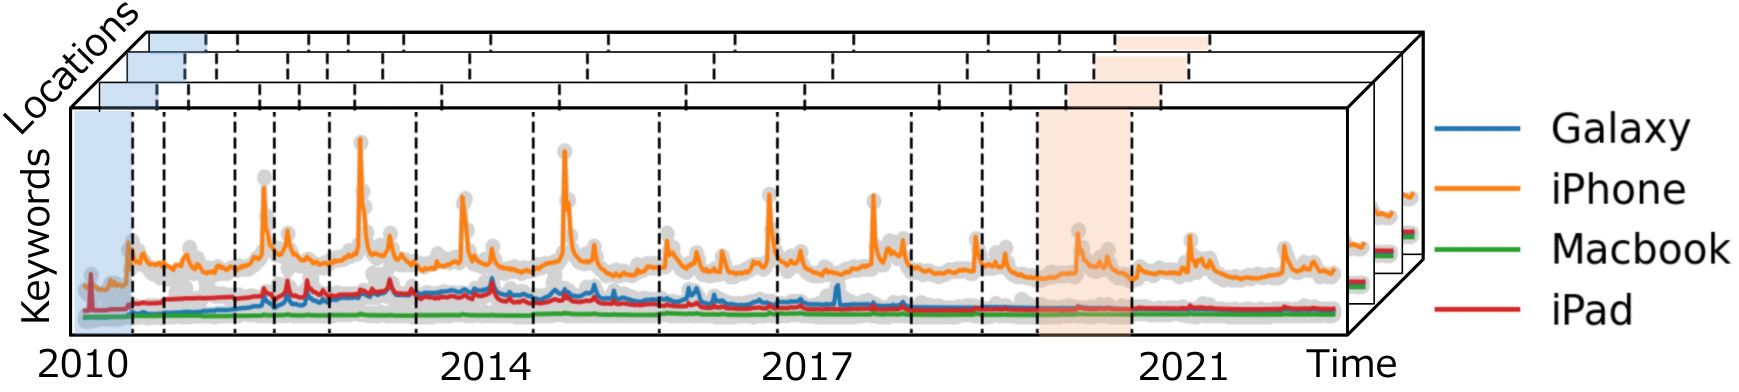
\includegraphics[width=\linewidth]{figures/Figure1_a.png}
    \caption{Dữ liệu thật (xám) và mô hình khớp (màu); các đường chấm dọc đánh dấu lúc đổi mô hình.}
  \end{subfigure}

  \vspace{4mm}
  \begin{subfigure}[t]{0.82\linewidth}
    \centering
    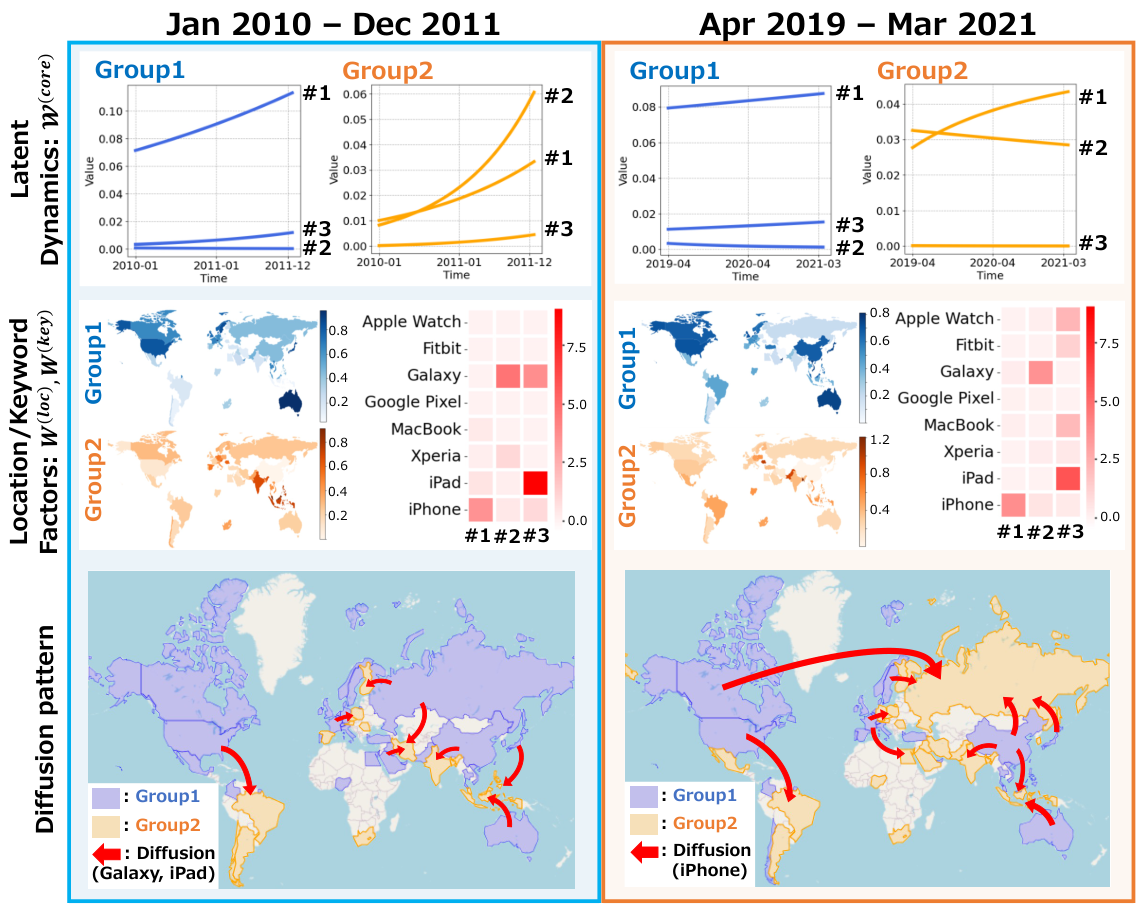
\includegraphics[width=\linewidth]{figures/Figure1_b.png}
    \caption{Lõi dynamics, hệ số địa điểm/từ khóa và bản đồ lan truyền ở hai giai đoạn.}
  \end{subfigure}
  \caption{Sức mạnh mô hình hóa của D-Tracker trên dữ liệu thiết bị. Nguồn: Higashiguchi et al.
  (2025), arXiv:2505.00242v1, Figure~1; hình của tác giả, CC BY 4.0.}
  \label{fig:preview}
\end{figure}

Ở Hình~\ref{fig:preview}(a), mô hình không dùng một bộ tham số cho toàn bộ giai đoạn hiển thị. Các đường
chấm cho thấy nó chia stream thành nhiều giai đoạn và dùng một mô hình cho mỗi giai đoạn. Đây là
cơ chế \emph{regime switching}. Ở Hình~\ref{fig:preview}(b), mỗi cột là một dynamics: đường
trên cùng là lõi $\mathcal{W}^{(\mathrm{core})}$ theo thời gian; hàng giữa là mức liên hệ của
dynamics với các từ khóa và nhóm địa điểm; hàng dưới là mũi tên lan truyền giữa các nhóm. Nhờ
vậy, ta không chỉ có một con số dự báo mà còn có một câu chuyện có thể kiểm tra: dynamics nào,
từ khóa nào, khu vực nào, lan theo hướng nào.

\begin{figure}[htbp]
  \centering
  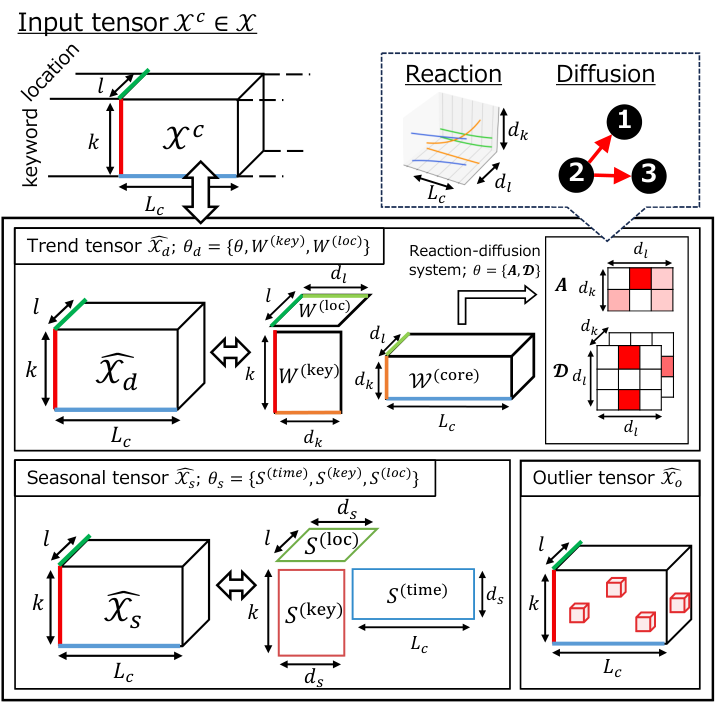
\includegraphics[width=0.72\linewidth]{figures/overview.png}
  \caption{Tổng quan D-Tracker: tensor hiện tại xấp xỉ bằng trend + seasonal + outlier. Nguồn:
  Higashiguchi et al. (2025), arXiv:2505.00242v1, Figure~2; hình của tác giả, CC BY 4.0.}
  \label{fig:overview}
\end{figure}

Hình~\ref{fig:overview} là bản đồ toàn bài. Đầu vào là tensor hiện tại $\mathcal{X}^{c}$.
Ba nhánh tương ứng ba giả định: phần thay đổi chậm/lan truyền, phần lặp theo mùa, và phần bất
thường thưa. Chương~\ref{sec:model} sẽ giải thích vì sao phần trend được nén thành lõi nhỏ và
vì sao lõi đó có thể sinh ra bằng một hệ phương trình vi phân.

\begin{selfcheck}
\begin{enumerate}
  \item Vì sao một mô hình duy nhất cho toàn bộ stream có thể thất bại dù dữ liệu lịch sử rất nhiều?
  \item Ba thành phần trend, seasonal, outlier trả lời ba câu hỏi nào ở đầu chương?
  \item ``Diễn giải được'' của D-Tracker dựa trên cấu trúc nào, và nó \emph{không} khẳng định điều gì?
\end{enumerate}
\end{selfcheck}

\section{Dữ liệu tensor stream và bài toán dự báo}
\label{sec:problem}

\subsection{Từ bảng đến tensor}

Một chuỗi thời gian thông thường có dạng $x_1,x_2,\ldots,x_T$: một giá trị tại mỗi thời điểm.
Dữ liệu của D-Tracker có thêm hai chiều. Với $k$ từ khóa, $l$ địa điểm và $t$ thời điểm, mỗi
lát cắt thời gian là một \emph{ma trận} $X_t\in\mathbb{R}^{k\times l}$, trong đó
$x_{ij}(t)$ là mức quan tâm của từ khóa $i$ tại địa điểm $j$ ở thời điểm $t$. Ghép các ma trận
lại, ta có tensor bậc ba
\begin{equation}
  \mathcal{X}=\{X_1,\ldots,X_{t_c}\}\in\mathbb{N}^{k\times l\times t_c},
  \label{eq:stream}
\end{equation}
với $t_c$ là thời điểm hiện tại. Paper hiển thị tensor thực nghiệm theo thứ tự thời gian, từ khóa,
địa điểm; khi viết công thức, tác giả dùng các chiều $k,l,L_c$. Hai cách viết mô tả cùng một đối
tượng, chỉ khác thứ tự trục.

\begin{center}
\small
\begin{tabular}{@{}lll@{}}
  \toprule
  Ký hiệu & Ý nghĩa & Ví dụ \\
  \midrule
  $k$ & số từ khóa & iPhone, Galaxy, iPad \\
  $l$ & số địa điểm & Hoa Kỳ, Việt Nam, Nhật Bản \\
  $t_c$ & thời điểm hiện tại & tuần thứ 676 \\
  $L_c$ & độ dài cửa sổ hiện tại & 104 tuần (hai năm) \\
  $L_f$ & tầm dự báo & 13, 26 hoặc 39 tuần \\
  \bottomrule
\end{tabular}
\end{center}

\subsection{Stream: dữ liệu không có điểm kết thúc}

Trong ứng dụng thật, mỗi tuần ta nhận thêm một ma trận $X_{t_c+1}$. Không thể giữ toàn bộ lịch
sử mãi mãi, và mô hình cũ có thể không còn đúng. Paper định nghĩa \emph{cửa sổ hiện tại} bằng
$L_c$ lát cắt gần nhất. Bài in công thức với hai đầu mút
$\{X_t\}_{t=t_c-L_c}^{t_c}$; nếu hiểu cả hai đầu mút theo nghĩa bao gồm thì đó là $L_c+1$ lát cắt,
nên tài liệu dùng dạng nhất quán với độ dài đã nêu:
\begin{equation}
  \mathcal{X}^{c}=\{X_{t_c-L_c+1},\ldots,X_{t_c}\},
  \label{eq:window}
\end{equation}
gồm đúng $L_c$ lát cắt. Đây là điểm rất quan trọng: D-Tracker không học lại từ toàn bộ
stream ở mỗi bước. Nó ước lượng lại trên cửa sổ hiện tại, rồi dùng cơ chế cập nhật để quyết định
có thêm một mô hình mới vào bộ mô hình hay không.

\begin{center}
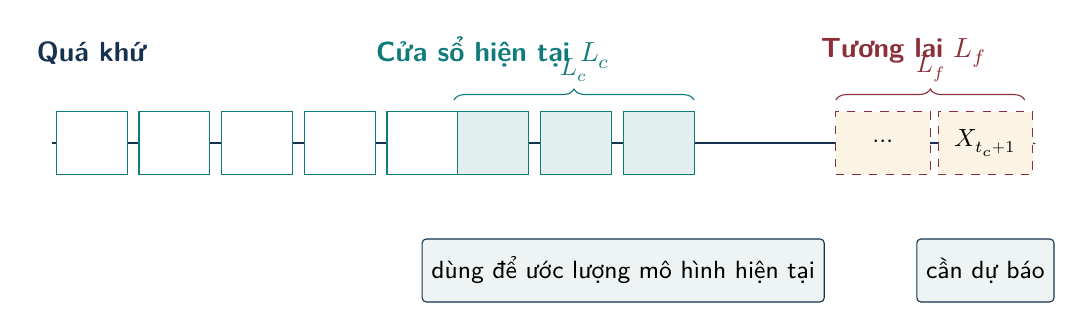
\begin{tikzpicture}[
  >=Latex,
  box/.style={draw=DTNavy, fill=DTMist, rounded corners=1.5pt,
              minimum height=8mm, align=center, font=\sffamily\small},
  obs/.style={draw=DTTeal, fill=white, minimum width=9mm, minimum height=8mm,
              align=center, font=\small},
  future/.style={draw=DTClaret, dashed, fill=DTWarm, minimum width=12mm,
                 minimum height=8mm, align=center, font=\small}
]
  \node[font=\sffamily\bfseries\color{DTNavy}] at (0,1.15) {Quá khứ};
  \node[font=\sffamily\bfseries\color{DTTeal}] at (5.1,1.15) {Cửa sổ hiện tại $L_c$};
  \node[font=\sffamily\bfseries\color{DTClaret}] at (10.3,1.15) {Tương lai $L_f$};
  \draw[->, thick, DTNavy] (-0.5,0) -- (12,0);
  \foreach \x in {0,...,4} {
    \node[obs] (h\x) at (\x*1.05,0) {};
  }
  \foreach \x in {0,...,2} {
    \node[obs, draw=DTTeal, fill=DTTeal!12] (c\x) at (5.1+\x*1.05,0) {};
  }
  \node[future] (f1) at (10.05,0) {$\cdots$};
  \node[future] (f2) at (11.35,0) {$X_{t_c+1}$};
  \draw[decorate,decoration={brace,amplitude=4pt},DTTeal]
    (4.6,0.55) -- (7.65,0.55) node[midway,above=3pt,font=\small] {$L_c$};
  \draw[decorate,decoration={brace,amplitude=4pt},DTClaret]
    (9.45,0.55) -- (11.85,0.55) node[midway,above=3pt,font=\small] {$L_f$};
  \node[box, below=8mm of c1, xshift=6mm] {dùng để ước lượng mô hình hiện tại};
  \node[box, below=8mm of f2] {cần dự báo};
\end{tikzpicture}
\end{center}

\subsection{Bài toán chính thức}

Paper phát biểu bài toán \emph{stream forecasting} như sau: cho cửa sổ $\mathcal{X}^{c}$ dài
$L_c$, hãy tìm các động học thay đổi theo thời gian gồm trend, mùa vụ và lan truyền, rồi dự báo
giá trị tại tầm $L_f$. Đầu ra là ma trận tại thời điểm đích
$\widehat{X}_{t_c+L_f}\in\mathbb{R}_{+}^{k\times l}$; khi đánh giá nhiều horizon, paper chạy từng
tầm riêng và không nói rằng mô hình phải sinh mọi ma trận trung gian.

\begin{keypoint}
\textbf{Đầu vào:} $L_c$ ma trận quan sát gần nhất, mỗi ma trận kích thước $k\times l$.\\
\textbf{Đầu ra:} dự báo tại thời điểm $t_c+L_f$, cùng một mô hình có các thành phần trend,
seasonal, outlier và lan truyền có thể đọc được.\\
\textbf{Ràng buộc:} không giữ toàn bộ stream; mỗi bước chỉ được xử lý trong thời gian không
phụ thuộc vào tổng chiều dài đã quan sát.
\end{keypoint}

Trong ví dụ ở Chương~\ref{sec:orientation}, $k=2$ (iPhone, Galaxy), $l=2$ (Hoa Kỳ, Việt Nam),
$L_c=3$ (ba tuần đã có), và $L_f=1$ nếu ta muốn dự báo tuần kế tiếp. Một mô hình tốt không chỉ
khớp ba tuần đó; nó phải tách được xu hướng của từng cặp và biểu diễn được việc mức quan tâm
có thể lan giữa hai địa điểm.

\subsection{Vì sao không dự báo từng chuỗi riêng lẻ?}

Ta có thể chạy một mô hình chuỗi thời gian cho từng cặp $(i,j)$. Cách đó bỏ qua hai điều:
\begin{itemize}
  \item các địa điểm và từ khóa chia sẻ những \emph{nhóm động học} tiềm ẩn; và
  \item dữ liệu có cấu trúc đa tuyến tính, nên một hệ số nhỏ có thể mô tả đồng thời nhiều cặp.
\end{itemize}
D-Tracker tìm một lõi nhỏ $\mathcal{W}^{(\mathrm{core})}$ và các hệ số địa điểm/từ khóa để tái tạo
toàn bộ tensor. Nhờ đó mô hình vừa giảm số tham số vừa tạo ra các nhóm có thể diễn giải. Cái giá
là phải giải một bài toán tối ưu khó hơn và phải kiểm tra giả định rằng cấu trúc nhóm đó thật sự
hữu ích.

\begin{plainwords}
Đừng nghĩ ``tensor'' là một khối dữ liệu bí ẩn. Hãy nghĩ đến một chồng bảng: mỗi tuần là một
bảng từ khóa $\times$ địa điểm. D-Tracker tìm một vài kiểu bảng chung, rồi trộn chúng với trọng
số khác nhau cho từng từ khóa và địa điểm.
\end{plainwords}

\begin{commonmistake}
Có hai nhầm lẫn thường gặp. Thứ nhất, tensor bậc ba không phải ``ba chiều không gian''; ba trục
ở đây là các thuộc tính dữ liệu. Thứ hai, mô hình không dự báo toàn bộ stream vô hạn cùng lúc:
nó chỉ dự báo $L_f$ bước từ cửa sổ hiện tại, rồi lặp lại khi có dữ liệu mới.
\end{commonmistake}

\subsection{Ba câu hỏi mà mô hình phải trả lời}

Paper đánh giá mô hình theo ba câu hỏi, và ta sẽ dùng chúng như khung đọc:
\begin{enumerate}
  \item \textbf{Accuracy:} dự báo tương lai chính xác đến đâu? (MAE, RMSE)
  \item \textbf{Scalability:} thời gian chạy thay đổi thế nào khi stream dài hơn?
  \item \textbf{Effectiveness:} mô hình có tách được trend, mùa vụ và lan truyền theo cách
        diễn giải được không?
\end{enumerate}
Ba câu hỏi này độc lập: một mô hình có thể khớp tốt nhưng không giải thích được, hoặc giải thích
đẹp nhưng dự báo kém. Toàn bộ thiết kế của D-Tracker là một nỗ lực cân bằng cả ba.

\begin{selfcheck}
\begin{enumerate}
  \item Với tensor $k=8,l=50,L_c=104$, mỗi lát cắt thời gian có bao nhiêu phần tử?
  \item Phân biệt $t_c$, $L_c$ và $L_f$ trong một câu.
  \item Tại sao chỉ dùng cửa sổ gần nhất lại giúp mô hình thích nghi với pattern thay đổi?
\end{enumerate}
\end{selfcheck}

\section{Kiến thức nền: tensor, phân rã và ba thành phần}
\label{sec:tensor-primer}

\subsection{Scalar, vector, ma trận, tensor}

Từ ``tensor'' nghe đáng sợ, nhưng với bài này chỉ cần hiểu là \emph{mảng nhiều chiều}. Bảng
dưới đây là toàn bộ kiến thức tối thiểu cần cho các công thức của paper.

\begin{center}
\small
\begin{tabular}{@{}llll@{}}
  \toprule
  Đối tượng & Bậc & Ký hiệu ví dụ & Cách đọc \\
  \midrule
  Scalar & 0 & $x=7$ & một số \\
  Vector & 1 & $\mathbf{w}=(w_1,\ldots,w_k)$ & danh sách theo từ khóa \\
  Ma trận & 2 & $\mathbf{W}\in\mathbb{R}^{k\times l}$ & bảng từ khóa $\times$ địa điểm \\
  Tensor & 3 & $\mathcal{X}\in\mathbb{R}^{k\times l\times L_c}$ & chồng bảng theo thời gian \\
  \bottomrule
\end{tabular}
\end{center}

Chỉ số được viết từ trái sang phải theo đúng thứ tự trục. Với tensor bậc ba, $x_{ij}(t)$ là phần
tử ở từ khóa $i$, địa điểm $j$, thời điểm $t$. Nếu $k=2,l=2,L_c=3$, tensor có $2\cdot2\cdot3=12$
phần tử. Phép ``unfold'' (trải phẳng) biến tensor thành ma trận bằng cách gộp một số trục; ví dụ
unfold theo trục từ khóa cho ta một ma trận để giải bằng đại số tuyến tính. Ta không cần tự làm
phép unfold bằng tay, nhưng cần hiểu nó chỉ là \emph{đổi cách xếp các số}, không tạo thêm dữ liệu.

\subsection{Phân rã Tucker bằng trực giác}

Giả sử ta có $k$ từ khóa và $l$ địa điểm. Thay vì lưu mọi giá trị của tensor, ta giả định dữ liệu
được tạo bởi một số ít \emph{kiểu động học} chung. Gọi $d_k$ là số nhóm từ khóa và $d_l$ là số
nhóm địa điểm, với $d_k\ll k$ và $d_l\ll l$. Khi đó, phần trend được xấp xỉ
\begin{equation}
  \widehat{\mathcal{X}}_d
  =\mathcal{W}^{(\mathrm{core})}
   \times_{\mathrm{key}}\mathbf{W}^{(\mathrm{key})}
   \times_{\mathrm{loc}}\mathbf{W}^{(\mathrm{loc})},
  \label{eq:tucker-intuition}
\end{equation}
trong đó $\mathcal{W}^{(\mathrm{core})}$ là một tensor nhỏ $d_k\times d_l\times L_c$, còn
$\mathbf{W}^{(\mathrm{key})}$ và $\mathbf{W}^{(\mathrm{loc})}$ là các bảng hệ số không âm kích
thước $d_k\times k$ và $d_l\times l$.

Ký hiệu $\times_{\mathrm{key}},\times_{\mathrm{loc}}$ gọi là \emph{mode product}. Có thể đọc
công thức~\eqref{eq:tucker-intuition} bằng lời như sau: lấy lõi nhỏ, trải nó ra theo các nhóm
từ khóa với trọng số $\mathbf{W}^{(\mathrm{key})}$, rồi trải theo các nhóm địa điểm với trọng số
$\mathbf{W}^{(\mathrm{loc})}$. Nếu một từ khóa có trọng số cao ở nhóm 2, nó sẽ nhận nhiều hơn
dynamics của nhóm 2. Nếu mọi trọng số đều không âm, việc trộn không đảo dấu của dynamics, nên
ta vẫn đọc được ``nhóm này tăng'' hay ``nhóm này giảm''.

\begin{keypoint}
Phân rã Tucker không phải là nén file tùy tiện. Nó tạo ra một lõi nhỏ chứa \emph{động học chung}
và các hệ số nói \emph{thành viên nào thuộc nhóm nào}. Đây là cầu nối giữa dự báo và diễn giải.
\end{keypoint}

\subsection{Ví dụ \texorpdfstring{$2\times2\times3$}{2x2x3} và lợi ích nén}

Hãy tưởng tượng hai từ khóa, hai địa điểm, ba tuần. Raw tensor có 12 số. Nếu giả sử chỉ có một
nhóm từ khóa và một nhóm địa điểm ($d_k=d_l=1$), lõi có $1\cdot1\cdot3=3$ số, hai hệ số có
$1\cdot2+1\cdot2=4$ số: tổng 7 tham số thay cho 12. Với dữ liệu thật, khoảng cách lớn hơn nhiều.
Một cửa sổ Device có $8\cdot50\cdot104=41{,}600$ phần tử. Với $d_k=3,d_l=2$, lõi có
$3\cdot2\cdot104=624$ phần tử và hai hệ số có $3\cdot8+2\cdot50=124$ phần tử: khoảng 748 tham số,
chưa bằng 2\% kích thước cửa sổ.

\begin{plainwords}
Nén ở đây không phải để tiết kiệm ổ đĩa. Mục đích là buộc mô hình giải thích hàng chục nghìn
quan sát bằng một vài dynamics và một bảng ``ai thuộc nhóm nào''. Nếu mô hình vẫn khớp tốt, cấu
trúc nhóm là một giả thuyết có ích.
\end{plainwords}

\subsection{Trend, seasonal và outlier trong một chuỗi nhỏ}

Ba thành phần trong D-Tracker cộng lại xấp xỉ dữ liệu:
\begin{equation}
  \mathcal{X}^{c}\approx\widehat{\mathcal{X}}_d
  +\widehat{\mathcal{X}}_s+\widehat{\mathcal{X}}_o.
  \label{eq:decompose-primer}
\end{equation}
Bảng~\ref{tab:three-components} là ví dụ số \textbf{do tài liệu tạo}. Dòng ``quan sát'' bằng
đúng tổng ba dòng còn lại; dấu gạch ngang ở outlier nghĩa là 0.

\begin{table}[htbp]
  \centering
  \small
  \caption{Ví dụ minh họa phép cộng trend + seasonal + outlier.}
  \label{tab:three-components}
  \begin{tabular}{lrrrrrrrr}
    \toprule
    Thành phần & Tuần 1 & 2 & 3 & 4 & 5 & 6 & 7 & 8 \\
    \midrule
    Quan sát      & 10 & 12 & 15 & 14 & 11 & 13 & 17 & 25 \\
    Trend         & 10 & 11 & 12 & 13 & 14 & 15 & 16 & 17 \\
    Seasonal      &  0 &  1 &  3 &  1 & $-3$ & $-2$ &  1 &  3 \\
    Outlier       &  -- & -- & -- & -- & -- & -- & -- &  5 \\
    \bottomrule
  \end{tabular}
\end{table}

Trend là phần thay đổi tương đối mượt. Seasonal là phần lặp lại có chu kỳ (ở đây minh họa bằng
một pattern ngắn; dữ liệu thật dùng chu kỳ tuần/năm). Outlier là phần bất thường và được giả định
\emph{thưa}: chỉ một số ít ô khác 0. Tách như vậy giúp mô hình không dùng một cú tăng đột biến
để kết luận rằng cả xu hướng đã thay đổi.

\subsection{Từ phân rã đến câu hỏi của paper}

Ta đã có ba mảnh: một tensor quan sát, một cách nén trend bằng lõi và hệ số, và một phép tách
thành ba thành phần. Paper thêm hai ý tưởng nữa:
\begin{itemize}
  \item lõi trend không tiến hóa tùy ý, mà tuân theo một hệ \textbf{reaction--diffusion}; và
  \item mô hình được cập nhật theo stream, với cấu trúc (số nhóm) và thời điểm đổi mô hình được
        chọn tự động.
\end{itemize}
Chương~\ref{sec:reaction-diffusion} giải thích ý tưởng thứ nhất; Chương~\ref{sec:model} ghép tất
cả lại thành mô hình hoàn chỉnh.

\begin{commonmistake}
Ba lỗi hiểu thường gặp: (1) coi $\mathcal{W}^{(\mathrm{core})}$ là tensor dữ liệu gốc thu nhỏ ---
nó là \emph{tham số ẩn} được học; (2) coi hệ số $\mathbf{W}$ là xác suất --- chúng là trọng số
không âm, không nhất thiết cộng lại bằng 1; (3) coi phép tách là duy nhất --- các phép phân rã
tensor thường chỉ xác định tới một phép biến đổi, và paper giải một bài tối ưu cụ thể.
\end{commonmistake}

\begin{selfcheck}
\begin{enumerate}
  \item Với $d_k=2,d_l=3,L_c=10$, lõi có bao nhiêu phần tử?
  \item Giải thích bằng một câu vì sao hệ số không âm giúp giữ chiều của dynamics.
  \item Trong bảng ba thành phần, nếu bỏ outlier ở tuần 8 thì mô hình sẽ hiểu sai điều gì?
\end{enumerate}
\end{selfcheck}

\section{Reaction--diffusion: vì sao mức quan tâm lan truyền?}
\label{sec:reaction-diffusion}

\subsection{Hai bể nước và một ý tưởng}

Trong hóa học, một chất khuếch tán từ nơi có nồng độ cao sang nơi có nồng độ thấp. D-Tracker
mượn hình ảnh đó cho mức quan tâm: nếu một từ khóa đang được chú ý mạnh ở nhóm địa điểm $j'$,
sự chú ý có thể chảy sang nhóm $j$ đang thấp hơn. Phương trình reaction--diffusion tổng quát mà
paper dẫn ra có dạng
\begin{equation}
  \frac{\partial u_i}{\partial t}
  =f(u_i)+\sum_j D\,(u_j-u_i),
  \label{eq:rd-background}
\end{equation}
trong đó $u_i$ là nồng độ tại vị trí $i$ và $D$ là độ mạnh khuếch tán. Số hạng $f(u_i)$ được gọi
là \textbf{reaction}: nó mô tả thay đổi cục bộ tại chỗ. Số hạng $\sum_j D(u_j-u_i)$ là
\textbf{diffusion}: nó chỉ khác 0 khi các vị trí có mức khác nhau, và dấu của nó cho biết dòng
chảy vào hay ra.

\begin{center}
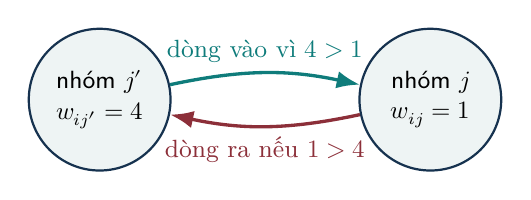
\begin{tikzpicture}[
  >=Latex,
  place/.style={circle, draw=DTNavy, thick, minimum size=18mm, fill=DTMist,
                align=center, font=\sffamily\small},
  flow/.style={->, very thick, DTTeal},
  label/.style={font=\small, align=center}
]
  \node[place] (b) at (0,0) {nhóm $j'$\\$w_{ij'}=4$};
  \node[place] (a) at (4.2,0) {nhóm $j$\\$w_{ij}=1$};
  \draw[flow] (b) to[bend left=12] node[above,label] {dòng vào vì $4>1$} (a);
  \draw[flow, DTClaret] (a) to[bend left=12] node[below,label] {dòng ra nếu $1>4$} (b);
\end{tikzpicture}
\end{center}

\subsection{Phiên bản latent của D-Tracker}

D-Tracker không áp đặt phương trình lên từng cặp từ khóa--địa điểm. Nó áp đặt lên \emph{lõi ẩn}
gồm $d_k\cdot d_l$ dynamics. Với $i=1,\ldots,d_k$ là nhóm từ khóa và $j=1,\ldots,d_l$ là nhóm
địa điểm, paper viết
\begin{equation}
  \frac{dw_{ij}}{dt}
  =a_{ij}w_{ij}
   +\sum_{j'=1}^{d_l} d_{ijj'}\,(w_{ij'}-w_{ij}),
  \qquad 1\leq i\leq d_k,\;1\leq j\leq d_l.
  \label{eq:rd-latent}
\end{equation}
Hai tham số mới cần đọc đúng:
\begin{itemize}
  \item $a_{ij}$ là \textbf{tốc độ tăng trưởng}. Nếu $a_{ij}>0$, dynamics $w_{ij}$ có xu hướng
        tăng; nếu $a_{ij}<0$, nó có xu hướng giảm. Đây là ``reaction''.
  \item $d_{ijj'}$ là \textbf{độ mạnh khuếch tán} từ nhóm địa điểm $j'$ sang nhóm $j$. Trong paper,
        $\mathcal{D}\in\mathbb{R}_{+}^{d_k\times d_l\times d_l}$ được mô tả là không âm. Dấu của
        dòng chảy thực tế còn phụ thuộc vào $(w_{ij'}-w_{ij})$: nếu $w_{ij'}>w_{ij}$ thì $j$ nhận
        thêm; nếu nhỏ hơn thì $j$ mất bớt.
\end{itemize}

Ở đây $w_{ij}$ là mức hoạt động của dynamics thuộc nhóm từ khóa $i$ và nhóm địa điểm $j$. Các
dynamics khác nhóm từ khóa không khuếch tán trực tiếp trong số hạng này; chúng tương tác qua lõi
và qua phép chiếu đa tuyến tính ở Chương~\ref{sec:model}. Toàn bộ hệ có $d_k\cdot d_l$ phương
trình, tham số gồm ma trận $\mathbf{A}\in\mathbb{R}^{d_k\times d_l}$ và tensor
$\mathcal{D}\in\mathbb{R}_{+}^{d_k\times d_l\times d_l}$.

\begin{keypoint}
$w>0$ giúp đọc ``mức hoạt động''; $a$ nói tăng hay giảm; $(w_{j'}-w_j)$ nói hướng chảy; $d$ nói
dòng chảy mạnh đến đâu. Đây là lý do mô hình có thể diễn giải được, chứ không chỉ là một hộp đen
dự báo.
\end{keypoint}

\subsection{Một bước số cụ thể}

Giả sử một dynamics ở nhóm $j$ có $w_j=1$, một dynamics cùng nhóm từ khóa ở nhóm $j'$ có
$w_{j'}=4$, $a_j=0.1$ và $d_{jj'}=0.5$. Bỏ qua các nhóm khác, đạo hàm tại thời điểm này là
\[
  \frac{dw_j}{dt}=0.1\cdot1+0.5\cdot(4-1)=0.1+1.5=1.6.
\]
Nếu xấp xỉ Euler với bước $\Delta t=1$, giá trị kế tiếp xấp xỉ $1+1.6=2.6$. Dynamics đang tăng
vì vừa có growth vừa nhận dòng từ nơi cao hơn. Nếu đổi $w_{j'}=0$, số hạng khuếch tán thành
$0.5(0-1)=-0.5$: cùng một độ mạnh $d$ nhưng dòng chảy đổi chiều.

\begin{plainwords}
Đừng học thuộc phương trình. Hãy đọc ba câu: ``tự nó tăng/giảm'', ``nó bị kéo về phía nhóm khác'',
và ``mức chênh càng lớn thì lực kéo càng mạnh''. Tất cả nằm trong hai số hạng của
Công thức~\eqref{eq:rd-latent}.
\end{plainwords}

\subsection{Liên hệ với dữ liệu quan sát}

Lõi $w_{ij}$ là ẩn. Để nối nó với chuỗi quan sát $X_{uv}$ của từ khóa thật $u$ và địa điểm thật
$v$, paper lấy đạo hàm của phép chiếu và thu được
\begin{equation}
  \frac{dX_{uv}}{dt}
  =\sum_{i=1}^{d_k}\sum_{j=1}^{d_l}
   W^{(\mathrm{key})}_{iu}W^{(\mathrm{loc})}_{jv}
   \underbrace{\left(
     a_{ij}w_{ij}+\sum_{j'=1}^{d_l}d_{ijj'}(w_{ij'}-w_{ij})
   \right)}_{\text{hệ reaction--diffusion ẩn}}.
  \label{eq:observed-derivative}
\end{equation}
Đọc từ phải sang trái: hệ ẩn tạo ra $d_k d_l$ động học; các trọng số không âm
$W^{(\mathrm{key})}_{iu}W^{(\mathrm{loc})}_{jv}$ quyết định dynamics nào đóng góp vào cặp
$(u,v)$. Vì trọng số không âm, phép chiếu không đảo dấu: một dynamics tăng vẫn đóng góp dương
vào chuỗi quan sát tương ứng. Đây là cầu nối giữa ``lõi nhỏ'' và ``chuỗi thật''.

\subsection{Diễn giải không đồng nghĩa với nhân quả}

Giả định reaction--diffusion nói rằng mức chênh có thể tạo ra dòng chảy. Mô hình học các tham số
$a,d$ và hệ số nhóm để khớp dữ liệu; nó \emph{không} chứng minh rằng sự tăng ở Mỹ gây ra sự tăng
ở Việt Nam. Một yếu tố thứ ba (ra mắt sản phẩm toàn cầu, tin tức, mạng xã hội) có thể tạo ra cùng
một pattern trễ. Vì vậy, hãy đọc kết quả là \textbf{giả thuyết lan truyền có cấu trúc}, cần kiểm
tra bằng kiến thức miền và thí nghiệm bổ sung.

\begin{commonmistake}
``$d_{ijj'}>0$ nghĩa là $j'$ luôn truyền sang $j$'' là chưa đủ. Dòng chảy còn phụ thuộc vào
$w_{ij'}-w_{ij}$; nếu $w_{ij'}<w_{ij}$, số hạng này âm. Paper gọi $d$ là độ mạnh, không phải một
chiều cố định. Tương tự, ``$a>0$'' chỉ nói xu hướng cục bộ, không đảm bảo tăng mãi mãi.
\end{commonmistake}

\begin{selfcheck}
\begin{enumerate}
  \item Với $w_j=2,w_{j'}=5,a_j=0,d_{jj'}=0.2$, đạo hàm bằng bao nhiêu?
  \item Nếu $a_{ij}<0$ và dòng khuếch tán dương, dynamics có chắc chắn giảm không? Vì sao?
  \item Nêu một tình huống dữ liệu có độ trễ giữa hai nơi nhưng không phải lan truyền nhân quả.
\end{enumerate}
\end{selfcheck}

\section{Mô hình D-Tracker hoàn chỉnh}
\label{sec:model}

\subsection{Ba thành phần cộng lại}

Với cửa sổ hiện tại $\mathcal{X}^{c}$, paper giả định dữ liệu quan sát là xấp xỉ tổng của một
tensor trend, một tensor seasonal và một tensor outlier (Eq.~(1) trong paper):
\begin{equation}
  \mathcal{X}^{c}\;\approx\;\widehat{\mathcal{X}}_d
  +\widehat{\mathcal{X}}_s+\widehat{\mathcal{X}}_o,
  \qquad
  \widehat{\mathcal{X}}_d,\widehat{\mathcal{X}}_s,\widehat{\mathcal{X}}_o
  \in\mathbb{R}^{k\times l\times L_c}.
  \label{eq:model-sum}
\end{equation}
Mục đích của phép tách không phải là trang trí. Mỗi thành phần có một giả định riêng:
\begin{itemize}
  \item $\widehat{\mathcal{X}}_d$ chứa \textbf{trend và diffusion}, phần thay đổi có cấu trúc;
  \item $\widehat{\mathcal{X}}_s$ chứa \textbf{mùa vụ}, phần lặp lại theo chu kỳ;
  \item $\widehat{\mathcal{X}}_o$ chứa \textbf{outlier}, phần bất thường và được giả định thưa.
\end{itemize}
Nếu không tách, một đợt khuyến mãi có thể bị học như một xu hướng dài hạn; nếu không có outlier,
một cú sốc có thể làm hỏng mọi hệ số.

\subsection{Trend: nén lõi và chiếu trở lại}

Tensor trend vẫn có kích thước $k\times l\times L_c$, quá lớn để đọc trực tiếp. Paper phân rã nó
thành một lõi nhỏ và hai bảng hệ số (Eq.~(2) trong paper):
\begin{equation}
  \widehat{\mathcal{X}}_d
  =\mathcal{W}^{(\mathrm{core})}
   \times_{\mathrm{key}}\mathbf{W}^{(\mathrm{key})}
   \times_{\mathrm{loc}}\mathbf{W}^{(\mathrm{loc})},
  \label{eq:trend-factorization}
\end{equation}
với
\[
  \mathcal{W}^{(\mathrm{core})}\in\mathbb{R}^{d_k\times d_l\times L_c},
  \quad
  \mathbf{W}^{(\mathrm{key})}\in\mathbb{R}_{+}^{d_k\times k},
  \quad
  \mathbf{W}^{(\mathrm{loc})}\in\mathbb{R}_{+}^{d_l\times l},
\]
và $d_k\ll k$, $d_l\ll l$. Viết theo từng phần tử, công thức này là
\begin{equation}
  \widehat{x}_{d,uv}(t)
  =\sum_{i=1}^{d_k}\sum_{j=1}^{d_l}
    w^{(\mathrm{core})}_{ij}(t)\,
    W^{(\mathrm{key})}_{iu}W^{(\mathrm{loc})}_{jv}.
  \label{eq:trend-elementwise}
\end{equation}
Từng ký hiệu có nghĩa rất cụ thể: $u$ là từ khóa thật, $v$ là địa điểm thật, $i,j$ là nhóm ẩn.
Nếu $W^{(\mathrm{key})}_{iu}$ lớn, từ khóa $u$ ``thuộc về'' nhóm $i$; nếu
$W^{(\mathrm{loc})}_{jv}$ lớn, địa điểm $v$ thuộc nhóm $j$. Lõi $w^{(\mathrm{core})}_{ij}(t)$ là
đường hoạt động của cặp nhóm đó.

\begin{keypoint}
Đẳng thức~\eqref{eq:trend-elementwise} là trái tim của khả năng diễn giải: giá trị thật của một
cặp $(u,v)$ bằng tổng các dynamics ẩn, mỗi dynamics được nhân với mức liên hệ của từ khóa và địa
điểm. Hệ số không âm giữ cho phép cộng không đảo chiều.
\end{keypoint}

\subsection{Lõi được sinh bởi hệ reaction--diffusion}

Paper không cho $w^{(\mathrm{core})}_{ij}(t)$ biến đổi tự do. Nó giả định lõi được sinh bởi hệ
phương trình~\eqref{eq:rd-latent} ở Chương~\ref{sec:reaction-diffusion}, tức Eq.~(3) trong paper:
\begin{equation}
  \frac{dw_{ij}}{dt}
  =a_{ij}w_{ij}
   +\sum_{j'=1}^{d_l}d_{ijj'}(w_{ij'}-w_{ij}).
  \label{eq:core-ode}
\end{equation}
Đây là một hệ \textbf{phương trình vi phân thường (ODE)} theo thời gian. Dữ liệu được quan sát
theo các bước rời rạc (tuần hoặc ngày), nhưng mô hình định nghĩa động học liên tục theo $t$ rồi
tích phân để tạo ra chuỗi $L_c$ bước. Điểm cần nhớ: vị trí là rời rạc (các nhóm địa điểm), còn
thời gian trong phương trình là liên tục.

Gọi $\theta=\{\mathbf{A},\mathcal{D}\}$ là tham số của hệ, và $w_0\in\mathbb{R}_{+}^{d_k\times d_l}$
là trạng thái ban đầu. Paper ký hiệu $f_\theta(\theta,w_0,L)$ là hàm sinh ra một chuỗi lõi dài $L$
từ $w_0$. Như vậy, phần trend hoàn chỉnh có tham số
\[
  \theta_d=\{\mathbf{W}^{(\mathrm{key})},\mathbf{W}^{(\mathrm{loc})},\theta\}.
\]
Nói cách khác, $\theta_d$ chứa cả ``các dynamics tiến hóa thế nào'' và ``các dynamics được gắn
với từ khóa/địa điểm nào''.

\subsection{Seasonal: một phép phân rã tương tự}

Phần mùa vụ cũng được nén, nhưng không dùng ODE. Paper phân rã (Eq.~(4)):
\begin{equation}
  \widehat{\mathcal{X}}_s
  =\mathbf{S}^{(\mathrm{time})}
   \times_{\mathrm{key}}\mathbf{S}^{(\mathrm{key})}
   \times_{\mathrm{loc}}\mathbf{S}^{(\mathrm{loc})},
  \label{eq:seasonal-factorization}
\end{equation}
với $d_s$ pattern mùa vụ và
\[
  \mathbf{S}^{(\mathrm{time})}\in\mathbb{R}^{d_s\times L_c},
  \quad
  \mathbf{S}^{(\mathrm{key})}\in\mathbb{R}^{d_s\times k},
  \quad
  \mathbf{S}^{(\mathrm{loc})}\in\mathbb{R}^{d_s\times l}.
\]
Theo từng phần tử:
\begin{equation}
  \widehat{x}_{s,uv}(t)
  =\sum_{r=1}^{d_s}
    S^{(\mathrm{time})}_{r,t}S^{(\mathrm{key})}_{r,u}S^{(\mathrm{loc})}_{r,v}.
  \label{eq:seasonal-elementwise}
\end{equation}
Mỗi $r$ là một ``khuôn'' mùa vụ theo thời gian; hai hệ số còn lại nói khuôn đó mạnh thế nào ở từng
từ khóa và địa điểm. Đây là dạng phân rã PARAFAC: mỗi pattern là một tổng hạng nhất (rank-one) của
ba vector. Paper không nói các hệ số mùa vụ bắt buộc không âm như $\mathbf{W}$ của trend, nên tài
liệu này không tự thêm ràng buộc đó.

\subsection{Outlier: thưa, không phải mọi nhiễu}

Tensor outlier $\widehat{\mathcal{X}}_o$ được giả định \emph{sparse}: hầu hết phần tử bằng 0, chỉ
giữ những giá trị bất thường không giải thích được bởi trend và mùa vụ. Trong tối ưu, paper tách
residual $\mathcal{X}^{c}-\widehat{\mathcal{X}}_d-\widehat{\mathcal{X}}_s$ và chỉ giữ các phần tử
làm giảm tổng chi phí MDL. Vì vậy ``outlier'' ở đây là một thành phần có cấu trúc, không phải
nhãn ``dữ liệu xấu''.

\subsection{Bộ tham số và nhiều regime}

Một mô hình đơn lẻ được gói trong
\[
  \Theta=\{\theta_d,\theta_s,\widehat{\mathcal{X}}_o\},
  \qquad
  \theta_s=\{\mathbf{S}^{(\mathrm{time})},\mathbf{S}^{(\mathrm{key})},
             \mathbf{S}^{(\mathrm{loc})}\}.
\]
Khi pattern thay đổi, một $\Theta$ không còn đủ. Paper cho phép dùng $N$ mô hình:
\[
  \mathcal{F}=\{\Theta_1,\Theta_2,\ldots,\Theta_N\}.
\]
Mỗi $\Theta_n$ mô tả một giai đoạn tương đối ổn định; $N$ và thời điểm chuyển được chọn tự động
bằng MDL ở Chương~\ref{sec:mdl-streaming}, không phải chia đoạn bằng mắt. Vì vậy, khi đọc một
hình như Hình~\ref{fig:preview}(a), các đường chấm dọc không phải sự kiện dữ liệu; chúng là ranh
giới của các mô hình.

\begin{center}
\small
\begin{tabular}{@{}p{0.24\linewidth}p{0.68\linewidth}@{}}
  \toprule
  Tham số & Chứa gì \\
  \midrule
  $\theta$ & $\mathbf{A}$ (growth) và $\mathcal{D}$ (diffusion) của hệ ẩn. \\
  $\theta_d$ & Lõi trend, hai bảng hệ số từ khóa/địa điểm và $\theta$. \\
  $\theta_s$ & Các pattern mùa vụ và hệ số từ khóa/địa điểm. \\
  $\Theta$ & Một mô hình đầy đủ: trend, mùa vụ và outlier. \\
  $\mathcal{F}$ & Tập nhiều $\Theta$, tương ứng các giai đoạn của stream. \\
  \bottomrule
\end{tabular}
\end{center}

\subsection{Đọc một dynamics từ lõi đến dữ liệu thật}

Giả sử mô hình học được $d_k=3$ nhóm từ khóa và $d_l=2$ nhóm địa điểm. Muốn hiểu ``Dynamics \#1
của Group 1'' trong Hình~\ref{fig:preview}(b), ta đi theo bốn bước:
\begin{enumerate}
  \item Xem đường lõi của dynamics đó đang tăng, giảm hay đổi hướng.
  \item Xem cột hệ số từ khóa tương ứng: từ khóa nào có trọng số cao? Trong ví dụ 2019--2021,
        paper cho thấy ``iPhone'' liên hệ mạnh với Dynamics \#1.
  \item Xem hàng hệ số địa điểm: nhóm nào có trọng số cao? Paper mô tả Group~1 gồm Hoa Kỳ, châu
        Âu và Trung Quốc; Group~2 là phần còn lại.
  \item Xem các $d_{ijj'}$ và dấu của $(w_{ij'}-w_{ij})$ để đọc hướng lan truyền. Paper mô tả
        Dynamics \#1 lan từ Group~1 sang Group~2, tức quan tâm ``iPhone'' lan từ các khu vực dẫn
        đầu ra phần còn lại của thế giới trong giai đoạn đó.
\end{enumerate}
Đây là \emph{diễn giải theo mô hình}, không phải nhãn do con người gán trước. Tên ``Group 1'' chỉ
có nghĩa sau khi học hệ số; nhóm không nhất thiết trùng với châu lục hay ngôn ngữ.

\begin{plainwords}
Muốn đọc kết quả, hãy tưởng tượng ba lớp: lõi nhỏ nói ``chuyện gì đang xảy ra'', hàng/cột hệ số
nói ``ở đâu và với từ khóa nào'', còn mũi tên diffusion nói ``đi từ nhóm nào sang nhóm nào''.
Bạn không cần nhìn toàn bộ tensor gốc.
\end{plainwords}

\begin{commonmistake}
Một lỗi phổ biến là đọc $d_l\ll k$ trong phần mô tả của paper như một ràng buộc thật. Kích thước
của $\mathbf{W}^{(\mathrm{loc})}$ là $d_l\times l$ và ý tưởng là giảm số nhóm địa điểm, nên tài
liệu dùng $d_k\ll k$, $d_l\ll l$. Đây là chỗ paper có khả năng đánh máy; ta nêu rõ thay vì lặng lẽ
sao chép. Một lỗi khác là coi $\Theta$ và $\mathcal{F}$ là một; $\mathcal{F}$ là \emph{tập} các
mô hình cho các giai đoạn khác nhau.
\end{commonmistake}

\begin{selfcheck}
\begin{enumerate}
  \item Viết kích thước của bốn đối tượng trong Công thức~\eqref{eq:trend-factorization}.
  \item Phân biệt $\theta$, $\theta_d$, $\Theta$ và $\mathcal{F}$ trong một câu mỗi ký hiệu.
  \item Vì sao seasonal không cần ODE reaction--diffusion? Nó khác trend ở giả định nào?
  \item Nếu $N=1$ trong toàn bộ stream, mô hình đang giả định điều gì?
\end{enumerate}
\end{selfcheck}

\section{Ước lượng tham số: vòng lặp ALS}
\label{sec:estimation}

\subsection{Bài toán tối ưu bằng trực giác}

Ta có dữ liệu $\mathcal{X}^{c}$ và một mô hình gồm nhiều khối: lõi trend, hệ reaction--diffusion,
hệ số từ khóa/địa điểm, hệ số mùa vụ và outlier. Nếu tối ưu tất cả cùng lúc, bài toán vừa phi
tuyến vừa nhiều tham số. Paper dùng \textbf{ALS} (alternating least squares): giữ phần lớn tham
số cố định, cập nhật một khối; lặp lại đến khi hội tụ.

\begin{keypoint}
ALS là chiến lược ``mỗi lần chỉ sửa một phần, nhưng sửa đến khi phần còn lại cho phép''. Nó không
đảm bảo tìm cực trị toàn cục cho bài toán không lồi; paper dùng nó như một thủ tục thực dụng và
báo cáo kết quả thực nghiệm.
\end{keypoint}

Để dễ theo dõi, tài liệu gọi sai số bình phương của một mô hình là
\begin{equation}
  \mathcal{L}(\Theta)
  =\left\|\mathcal{X}^{c}
    -\widehat{\mathcal{X}}_d-\widehat{\mathcal{X}}_s-\widehat{\mathcal{X}}_o
   \right\|_F^2.
  \label{eq:als-loss}
\end{equation}
Paper không đặt tên ký hiệu này trong mục 4.1, nhưng mọi bước cập nhật dưới đây đều nhằm giảm
sai số đó (hoặc giảm chi phí MDL ở bước outlier). Chuẩn Frobenius $\|\cdot\|_F$ chỉ là căn bậc hai
tổng bình phương mọi phần tử, tức một cách đo ``mô hình lệch dữ liệu bao nhiêu''.

\subsection{Khởi tạo: STL, PARAFAC và NTD}

Thuật toán ModelEstimation cần điểm bắt đầu. Paper mô tả ba bước khởi tạo:
\begin{enumerate}
  \item Dùng \textbf{STL} (seasonal-trend decomposition using LOESS) để tách cửa sổ hiện tại
        thành trend, seasonal và residual. STL là phương pháp thống kê cổ điển, mạnh với chuỗi
        có mùa vụ; nó cho ta xấp xỉ ban đầu của $\widehat{\mathcal{X}}_d$ và
        $\widehat{\mathcal{X}}_s$.
  \item Phân rã $\widehat{\mathcal{X}}_s$ bằng \textbf{PARAFAC} để có các hệ số mùa vụ ban đầu
        $\mathbf{S}^{(\mathrm{time})},\mathbf{S}^{(\mathrm{key})},\mathbf{S}^{(\mathrm{loc})}$.
  \item Áp dụng \textbf{Nonnegative Tucker Decomposition (NTD)} cho $\widehat{\mathcal{X}}_d$ để
        lấy $\mathbf{W}^{(\mathrm{key})},\mathbf{W}^{(\mathrm{loc})}$ ban đầu.
\end{enumerate}
Sau đó $\widehat{\mathcal{X}}_o$ được đặt bằng 0: giả định ban đầu là chưa có outlier. Việc khởi
tạo không phải chi tiết phụ; nó quyết định vòng ALS có rơi vào một nghiệm xấu hay không, và paper
ghi rõ cách làm trong Appendix A.1.

\subsection{Cập nhật hệ reaction--diffusion}

Giữ $\mathbf{W}^{(\mathrm{key})},\mathbf{W}^{(\mathrm{loc})}$ và các thành phần khác cố định,
paper giải bài toán bình phương tối thiểu phi tuyến
\begin{equation}
  \{\theta,w_0\}
  =\arg\min_{\theta',w_0'}
   \left\|
     \mathcal{X}^{c}-\widehat{\mathcal{X}}_s-\widehat{\mathcal{X}}_o
     -f_\theta(\theta',w_0',L_c)
       \times_{\mathrm{key}}\mathbf{W}^{(\mathrm{key})}
       \times_{\mathrm{loc}}\mathbf{W}^{(\mathrm{loc})}
   \right\|_F^2,
  \label{eq:lm-estimation}
\end{equation}
đây là Eq.~(5) trong paper. Ký hiệu $\arg\min$ nghĩa là ``chọn bộ tham số làm biểu thức nhỏ nhất''.
Vì $f_\theta$ chứa nghiệm của ODE, đạo hàm theo $\theta$ không có dạng đóng đơn giản. Paper dùng
\textbf{Levenberg--Marquardt (LM)}, một phương pháp số cho bình phương tối thiểu phi tuyến, để cập
nhật đồng thời các tham số $\mathbf{A},\mathcal{D}$ và trạng thái ban đầu $w_0$.

Ta không cần tự viết LM để hiểu paper, nhưng cần nhớ ba điều: (i) đây là bước đắt nhất về mặt
tính toán; (ii) nó cần một bộ giải ODE; (iii) kết quả phụ thuộc vào điểm khởi tạo và có thể chỉ là
cực trị địa phương.

\subsection{Cập nhật hệ số trend bằng multiplicative update}

Khi đã có lõi $\mathcal{W}^{(\mathrm{core})}$, paper cập nhật từng hệ số trend. Với
``mode'' là key hoặc loc, đặt
\begin{align}
  \mathbf{P}^{(\mathrm{mode})}
  &=\max\!\left(\epsilon,\;
    \mathbf{X}_d^{(\mathrm{mode})}\cdot\mathbf{G}^{(\mathrm{mode})}
   \right), \label{eq:w-p}\\
  \mathbf{Q}^{(\mathrm{mode})}
  &=\max\!\left(\epsilon,\;
    \mathbf{W}^{(\mathrm{mode})}\cdot\mathbf{G}^{(\mathrm{mode})}
    \cdot(\mathbf{G}^{(\mathrm{mode})})^{\mathsf T}
   \right), \label{eq:w-q}\\
  \mathbf{W}^{(\mathrm{mode})}
  &\leftarrow
    \mathbf{W}^{(\mathrm{mode})}
    \otimes\mathbf{P}^{(\mathrm{mode})}
    \oslash\mathbf{Q}^{(\mathrm{mode})}.
  \label{eq:multiplicative}
\end{align}
Đây là Eq.~(6) trong paper. Các ký hiệu:
\begin{itemize}
  \item $\mathbf{X}_d^{(\mathrm{mode})}$ là tensor residual
        $\mathcal{X}^{c}-\widehat{\mathcal{X}}_s-\widehat{\mathcal{X}}_o$ sau khi \emph{unfold}
        theo mode tương ứng (Eq.~7);
  \item $\mathbf{G}^{(\mathrm{mode})}$ là phần còn lại của phép chiếu, cũng được unfold;
  \item $\otimes$ là nhân từng phần tử (Hadamard), $\oslash$ là chia từng phần tử;
  \item $\epsilon$ là hằng số dương rất nhỏ để tránh chia cho 0.
\end{itemize}
Vì $\mathbf{W}$ ban đầu không âm và phép cập nhật chỉ nhân/chia các đại lượng dương, hệ số vẫn
không âm. Đây là lý do ``multiplicative'' quan trọng: nó vừa tối ưu vừa giữ ràng buộc.

\begin{plainwords}
Công thức~(6) nghe phức tạp, nhưng ý tưởng là: so sánh phần dữ liệu còn thiếu với phần mô hình
dự đoán, rồi tăng/giảm từng trọng số theo tỉ lệ. Không có phép trừ tự do nào có thể đẩy trọng số
xuống âm.
\end{plainwords}

\subsection{Cập nhật hệ số mùa vụ}

Với phần mùa vụ, paper giữ các thành phần khác cố định và dùng một bước ALS có dạng đóng. Với mỗi
mode trong $\{\mathrm{time},\mathrm{key},\mathrm{loc}\}$, đặt
\begin{align}
  \mathbf{U}^{(\mathrm{mode})}
  &=\odot_{i\neq\mathrm{mode}}\mathbf{S}^{(i)},&
  \mathbf{V}^{(\mathrm{mode})}
  &=\otimes_{i\neq\mathrm{mode}}
    (\mathbf{S}^{(i)})^{\mathsf T}\mathbf{S}^{(i)},\\
  \mathbf{S}^{(\mathrm{mode})}
  &\leftarrow
    \mathbf{X}_s^{(\mathrm{mode})}
    \mathbf{U}^{(\mathrm{mode})}
    (\mathbf{V}^{(\mathrm{mode})})^{\dagger}.
  \label{eq:seasonal-update}
\end{align}
Đây là Eq.~(8); $\odot$ và $\otimes$ lần lượt là tích Khatri--Rao và tích từng phần tử,
$\dagger$ là giả nghịch đảo Moore--Penrose, còn $\mathbf{X}_s^{(\mathrm{mode})}$ là residual
$\mathcal{X}^{c}-\widehat{\mathcal{X}}_d-\widehat{\mathcal{X}}_o$ được unfold (Eq.~9). Về bản
chất, đây là nghiệm bình phương tối thiểu tuyến tính khi giữ hai mode còn lại; không cần chứng
minh lại trong tài liệu này.

\subsection{Cập nhật outlier bằng sparsification}

Sau khi cập nhật trend và mùa vụ, residual còn lại là
$\mathcal{R}=\mathcal{X}^{c}-\widehat{\mathcal{X}}_d-\widehat{\mathcal{X}}_s$. Paper không dùng
một ngưỡng thủ công kiểu ``lớn hơn 3 thì là outlier''. Nó xét từng phần tử của $\mathcal{R}$ và
quyết định giữ hay đặt về 0 sao cho tổng chi phí MDL nhỏ nhất. Chi tiết chi phí ở
Chương~\ref{sec:mdl-streaming}; ở đây chỉ cần hiểu kết quả là một tensor thưa.

\subsection{Toàn bộ vòng lặp và độ phức tạp}

\begin{tcolorbox}[enhanced,breakable,colback=white,colframe=DTNavy,arc=1.5mm,
  title={\sffamily\bfseries Algorithm 2 --- ModelEstimation (tóm tắt)},fonttitle=\small,
  coltitle=white,colbacktitle=DTNavy,left=3mm,right=3mm,top=2mm,bottom=2mm]
\textbf{Input:} $\mathcal{X}^{c},d_k,d_l,d_s$.\quad
\textbf{Output:} $\Theta=\{\theta_d,\theta_s,\widehat{\mathcal{X}}_o\}$.
\begin{enumerate}[leftmargin=1.5em]
  \item Khởi tạo $\theta_d,\theta_s$ bằng STL + PARAFAC + NTD; đặt $\widehat{\mathcal{X}}_o=0$.
  \item \textbf{repeat}
  \item \quad Cập nhật $\theta=\{\mathbf{A},\mathcal{D}\}$ và $w_0$ bằng LM (Eq.~5).
  \item \quad Sinh $\mathcal{W}^{(\mathrm{core})}=f_\theta(\theta,w_0,L_c)$.
  \item \quad Cập nhật $\mathbf{W}^{(\mathrm{key})},\mathbf{W}^{(\mathrm{loc})}$ (Eq.~6).
  \item \quad Cập nhật $\mathbf{S}^{(\mathrm{time})},\mathbf{S}^{(\mathrm{key})},
        \mathbf{S}^{(\mathrm{loc})}$ (Eq.~8).
  \item \quad Sparsify residual để cập nhật $\widehat{\mathcal{X}}_o$.
  \item \textbf{until} hội tụ.
\end{enumerate}
\end{tcolorbox}

Lemma~1 (trong §4.1; HTML đặt nhãn là Lemma~4.1) phát biểu độ phức tạp thời gian của ModelEstimation là
\[
  O(d_k d_l^2+kd_k+ld_l).
\]
Con số này đến từ $d_k d_l^2$ tham số của hệ reaction--diffusion và chi phí cập nhật hai bảng hệ
số. Tuy nhiên, biểu thức đã bỏ qua số vòng lặp ALS, chi phí giải ODE, chi phí cập nhật mùa vụ và
outlier. Vì vậy, hãy đọc đây là độ phức tạp của \emph{một vòng cập nhật chính} theo cách paper
trình bày, không phải bảo đảm cho toàn bộ pipeline.

\begin{commonmistake}
``Hội tụ'' không có nghĩa tìm được nghiệm tốt nhất toàn cục. ALS trên bài toán không lồi có thể
dừng ở cực trị địa phương; paper không chứng minh tính tối ưu toàn cục. Ngoài ra, $\epsilon$ không
phải tham số mô hình cần học; nó chỉ bảo vệ phép chia.
\end{commonmistake}

\begin{selfcheck}
\begin{enumerate}
  \item Vì sao bước cập nhật $\theta$ cần LM thay vì một nghiệm đóng?
  \item Phép cập nhật nhân $\mathbf{W}\otimes\mathbf{P}\oslash\mathbf{Q}$ giữ được tính không âm nhờ đâu?
  \item Kể tên ba bước khởi tạo và phương pháp tương ứng.
  \item Độ phức tạp $O(d_kd_l^2+kd_k+ld_l)$ bỏ qua những chi phí nào?
\end{enumerate}
\end{selfcheck}

\section{MDL, chọn cấu trúc và streaming}
\label{sec:mdl-streaming}

\subsection{MDL bằng một hình ảnh rất đời thường}

Giả sử bạn phải gửi một file dữ liệu cho đồng nghiệp qua một kênh rất chậm. Bạn có hai cách:
gửi nguyên file, hoặc gửi một ``công thức mô tả file'' cộng với phần dữ liệu không khớp công thức.
Nếu công thức quá đơn giản, phần sai lệch còn lại rất lớn. Nếu công thức quá phức tạp, bản thân
công thức đã dài. \textbf{Minimum Description Length} (MDL) chọn cách mô tả có \emph{tổng số bit}
nhỏ nhất:
\begin{equation}
  \bigl\langle \mathcal{X};\mathcal{F}\bigr\rangle
  =\bigl\langle \mathcal{F}\bigr\rangle
   +\bigl\langle \mathcal{X}\mid\mathcal{F}\bigr\rangle.
  \label{eq:mdl-total}
\end{equation}
Đây là Eq.~(10) trong paper. Số hạng thứ nhất là chi phí mô tả mô hình; số hạng thứ hai là chi phí
mã hóa dữ liệu khi đã biết mô hình. Mô hình tốt không phải mô hình khớp tuyệt đối, mà là mô hình
giải thích được nhiều dữ liệu với ít bit.

\begin{keypoint}
MDL là một nguyên tắc cân bằng giữa \textbf{độ khớp} và \textbf{độ phức tạp}. Nó đồng thời dùng
để chọn số chiều ẩn, quyết định giữ outlier nào, và quyết định có thêm một regime mới hay không.
Vì vậy paper mới có thể nói mô hình ``tự động''.
\end{keypoint}

\subsection{Chi phí mô tả mô hình}

Với mỗi mô hình $\Theta$, paper tính chi phí từ các tham số khác 0. Gọi $|\cdot|$ là số phần tử
khác 0, $c_F=32$ là số bit cho một số thực, và $\log^*$ là độ dài mã phổ dụng cho một số nguyên.
Các công thức có cùng một khuôn:
\begin{align}
  \bigl\langle\mathcal{F}\bigr\rangle
  &=\sum_{\Theta\in\mathcal{F}}\bigl\langle\Theta\bigr\rangle,
  &
  \bigl\langle\Theta\bigr\rangle
  &=\bigl\langle\theta_d\bigr\rangle
   +\bigl\langle\theta_s\bigr\rangle
   +\bigl\langle\widehat{\mathcal{X}}_o\bigr\rangle,
  \label{eq:model-cost}\\
  \bigl\langle\mathbf{W}^{(\mathrm{key})}\bigr\rangle
  &=|\mathbf{W}^{(\mathrm{key})}|
    \bigl(\log d_k+\log k+c_F\bigr)
    +\log^*|\mathbf{W}^{(\mathrm{key})}|,
  \label{eq:cost-wkey}\\
  \bigl\langle\mathbf{W}^{(\mathrm{loc})}\bigr\rangle
  &=|\mathbf{W}^{(\mathrm{loc})}|
    \bigl(\log d_l+\log l+c_F\bigr)
    +\log^*|\mathbf{W}^{(\mathrm{loc})}|,\\
  \bigl\langle\theta\bigr\rangle
  &=\bigl\langle\mathbf{A}\bigr\rangle
   +\bigl\langle\mathcal{D}\bigr\rangle,\\
  \bigl\langle\mathbf{A}\bigr\rangle
  &=|\mathbf{A}|\bigl(\log d_k+\log d_l+c_F\bigr)
    +\log^*|\mathbf{A}|,\\
  \bigl\langle\mathcal{D}\bigr\rangle
  &=|\mathcal{D}|\bigl(\log d_k+2\log d_l+c_F\bigr)
    +\log^*|\mathcal{D}|.
  \label{eq:cost-theta}
\end{align}
Các hệ số mùa vụ và outlier có chi phí tương tự:
\begin{align}
  \bigl\langle\mathbf{S}^{(\mathrm{time})}\bigr\rangle
  &=|\mathbf{S}^{(\mathrm{time})}|
    \bigl(\log d_s+\log L_c+c_F\bigr)
    +\log^*|\mathbf{S}^{(\mathrm{time})}|,\\
  \bigl\langle\mathbf{S}^{(\mathrm{key})}\bigr\rangle
  &=|\mathbf{S}^{(\mathrm{key})}|
    \bigl(\log d_s+\log k+c_F\bigr)
    +\log^*|\mathbf{S}^{(\mathrm{key})}|,\\
  \bigl\langle\mathbf{S}^{(\mathrm{loc})}\bigr\rangle
  &=|\mathbf{S}^{(\mathrm{loc})}|
    \bigl(\log d_s+\log l+c_F\bigr)
    +\log^*|\mathbf{S}^{(\mathrm{loc})}|,\\
  \bigl\langle\widehat{\mathcal{X}}_o\bigr\rangle
  &=|\widehat{\mathcal{X}}_o|
    \bigl(\log n+\log k+\log l+c_F\bigr)
    +\log^*|\widehat{\mathcal{X}}_o|.
  \label{eq:cost-outlier}
\end{align}
Không cần thuộc từng dòng. Điều cần hiểu là: chi phí tăng theo số phần tử khác 0 và theo kích
thước các trục; do đó tăng $d_k,d_l,d_s$ làm mô hình đắt hơn, còn thêm outlier cũng làm mô hình
đắt hơn. Ký hiệu $n$ trong chi phí outlier không được định nghĩa lại ngay tại công thức; paper dùng
nó như độ dài stream/tổng số phần tử. Đây là một điểm chưa rõ của bài, nên tài liệu giữ nguyên
công thức và ghi chú thay vì tự gán nghĩa chắc chắn.

\subsection{Chi phí mã hóa dữ liệu}

Phần còn lại là chi phí mô tả dữ liệu dưới mô hình. Paper dùng mã Huffman và mô hình nhiễu Gauss
với trung bình $\mu$, phương sai $\sigma^2$:
\begin{equation}
  \bigl\langle\mathcal{X}\mid\mathcal{F}\bigr\rangle
  =\sum_{x\in\mathcal{X}}
   -\log_2 p_{\mu,\sigma}
   \bigl(x-\widehat{x}_d-\widehat{x}_s-\widehat{x}_o\bigr).
  \label{eq:data-cost}
\end{equation}
Đây là Eq. không số ngay sau Eq.~(10) trong paper. Trực giác: nếu residual
$x-\widehat{x}_d-\widehat{x}_s-\widehat{x}_o$ nhỏ và phù hợp với nhiễu dự kiến, nó tốn ít bit;
nếu residual lớn bất thường, nó tốn nhiều bit. Vì vậy mô hình vừa phải khớp, vừa không được biến
mọi dao động nhỏ thành tham số.

\begin{plainwords}
MDL không hỏi ``mô hình nào khớp nhất?''. Nó hỏi ``mô hình nào cho bản mô tả ngắn nhất của cả mô
hình lẫn dữ liệu?''. Một mô hình quá to có thể khớp hoàn hảo nhưng bản mô tả dài; một mô hình quá
nhỏ có bản mô tả ngắn nhưng phần residual dài. Điểm cân bằng chính là cấu trúc tối ưu.
\end{plainwords}

\subsection{Outlier và số chiều được chọn thế nào?}

Với outlier, paper thử đặt từng phần tử residual về 0 và giữ lại nếu tổng chi phí giảm. Đây là
``sparsification'' có tiêu chuẩn, không phải ngưỡng cảm tính.

Với số chiều, Algorithm~4 (\textsc{RankUpdate}) thử các cấu hình chỉ thay đổi một rank một đơn vị:
$(d_k-1,d_l,d_s)$, $(d_k+1,d_l,d_s)$, $(d_k,d_l-1,d_s)$, $(d_k,d_l+1,d_s)$,
$(d_k,d_l,d_s-1)$, $(d_k,d_l,d_s+1)$. Mỗi cấu hình được ước lượng lại, rồi giữ cấu hình có tổng
chi phí nhỏ nhất. Trong bản HTML/PDF của paper, danh sách candidate in ra lặp
$(d_k,d_l+1,d_s)$ và thiếu $(d_k+1,d_l,d_s)$; đây là lỗi trình bày có khả năng cao. Tài liệu dùng
danh sách đầy đủ theo ý tưởng ``mỗi lần đổi một rank'' và ghi chú rõ.

\subsection{ModelUpdate: thêm, giữ hay chuyển regime?}

Algorithm~3 so sánh tổng chi phí khi thêm candidate $\Theta'$ vào bộ mô hình $\mathcal{F}$ với
tổng chi phí khi không thêm. Nếu thêm làm chi phí giảm, candidate được chấp nhận; nếu không, mô
hình cũ được giữ. Sau khi chấp nhận, RankUpdate có thể điều chỉnh $d_k,d_l,d_s$.

\begin{center}
\resizebox{\textwidth}{!}{%
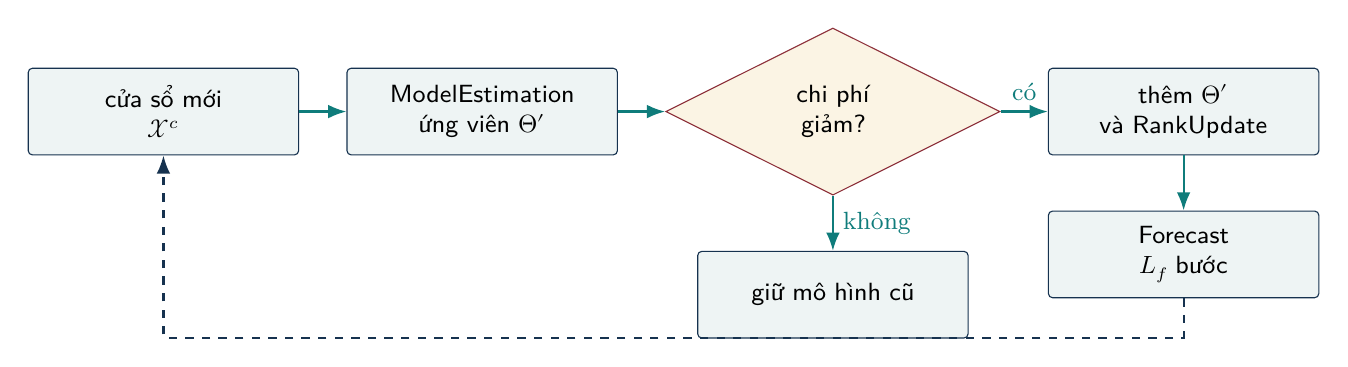
\begin{tikzpicture}[
  >=Latex,
  node distance=6mm and 6mm,
  stage/.style={draw=DTNavy, rounded corners=1.5pt, fill=DTMist,
    text width=3.2cm, minimum height=11mm, align=center, font=\sffamily\small},
  decision/.style={diamond, draw=DTClaret, fill=DTWarm, aspect=2.0,
    text width=2.2cm, align=center, font=\sffamily\small},
  arrow/.style={->, thick, DTTeal}
]
  \node[stage] (x) {cửa sổ mới\\$\mathcal{X}^{c}$};
  \node[stage, right=of x] (est) {ModelEstimation\\ứng viên $\Theta'$};
  \node[decision, right=of est] (cost) {chi phí\\giảm?};
  \node[stage, right=of cost] (add) {thêm $\Theta'$\\và RankUpdate};
  \node[stage, below=7mm of cost] (keep) {giữ mô hình cũ};
  \node[stage, below=7mm of add] (fc) {Forecast\\$L_f$ bước};
  \draw[arrow] (x) -- (est);
  \draw[arrow] (est) -- (cost);
  \draw[arrow] (cost) -- node[above,font=\small]{có} (add);
  \draw[arrow] (cost) -- node[right,font=\small]{không} (keep);
  \draw[arrow] (add) -- (fc);
  \draw[arrow, dashed, DTNavy] (fc.south) -- ++(0,-0.5) -| (x.south);
\end{tikzpicture}%
}
\end{center}

\subsection{Toàn bộ thuật toán streaming}

Algorithm~1 khởi tạo trên cửa sổ đầu tiên, đặt $\mathcal{F}=\{\Theta\}$, rồi với mỗi thời điểm
$t_c$:
\begin{enumerate}
  \item lấy cửa sổ $\mathcal{X}^{c}$;
  \item chạy ModelEstimation để có candidate $\Theta'$;
  \item chạy ModelUpdate để quyết định thêm/giữ và cập nhật rank;
  \item dự báo $L_f$ bước bằng $\mathcal{F}$;
  \item chuyển sang thời điểm kế tiếp.
\end{enumerate}

\begin{keypoint}
Chi phí mỗi bước không phụ thuộc vào tổng chiều dài stream vì bước 1 luôn lấy đúng $L_c$ lát cắt.
Tập $\mathcal{F}$ có thể tăng khi có regime mới, và RankUpdate tạo các ``spike'' thời gian, nhưng
không có vòng lặp trên toàn bộ lịch sử. Đây là ý nghĩa chính xác của scalability trong paper.
\end{keypoint}

\subsection{Forecast và những gì paper không nói}

Algorithm~1 gọi $\widehat{\mathcal{X}}_{t_c+L_f}=\mathrm{Forecast}(\mathcal{F})$ nhưng không trình
bày chi tiết công thức Forecast trong các mục chính. Vì vậy, tài liệu này chỉ nói điều chắc chắn:
dự báo dùng mô hình đang hoạt động trong $\mathcal{F}$, và trend có thể được ngoại suy từ hệ
reaction--diffusion. Ta \emph{không} tự bịa một công thức chi tiết cho seasonal/outlier. Nếu cần
tái hiện chính xác, phải đọc code gốc hoặc appendix/implementation của tác giả.

\subsection{``Parameter-free'' nghĩa là gì?}

Paper nói D-Tracker không cần chỉnh tham số. Cần đọc đúng ngữ cảnh: người dùng không phải chọn
tay số nhóm $d_k,d_l,d_s$ hay thời điểm đổi regime; các đại lượng đó được chọn bằng MDL. Tuy nhiên
vẫn có các lựa chọn kỹ thuật như bộ giải ODE, số vòng lặp ALS, dung sai hội tụ, và trong thí nghiệm
paper tìm kiếm khởi tạo $d_k,d_l\in[2,4]$, $d_s\in[0,4]$. ``Không hyperparameter'' không có nghĩa
``không có bất kỳ tham số số học nào''.

\begin{commonmistake}
Đừng nói ``MDL luôn tìm mô hình đúng''. MDL tối ưu một tiêu chuẩn mã hóa; nếu giả định nhiễu sai,
hoặc dữ liệu thật sự phức tạp hơn họ mô hình, mô hình tối ưu theo MDL vẫn có thể dự báo kém. Nó
cũng không thay thế kiểm định nhân quả cho các mũi tên diffusion.
\end{commonmistake}

\begin{selfcheck}
\begin{enumerate}
  \item Một mô hình tăng $d_k$ sẽ làm thành phần nào của MDL tăng, và có thể làm thành phần nào giảm?
  \item Vì sao outlier không được chọn bằng ngưỡng cố định?
  \item Nếu candidate model không làm giảm tổng chi phí, ModelUpdate làm gì?
  \item Giải thích trong một câu vì sao thời gian mỗi bước không tăng theo chiều dài stream.
\end{enumerate}
\end{selfcheck}

\section{Thí nghiệm: đọc kết quả mà không phóng đại}
\label{sec:experiments}

\subsection{Ba câu hỏi thực nghiệm}

Paper đánh giá D-Tracker bằng ba câu hỏi:
\begin{description}[leftmargin=1.8em,style=nextline]
  \item[Q1 --- Accuracy.] Dự báo tương lai chính xác đến đâu, so với các phương pháp mạnh?
  \item[Q2 --- Scalability.] Thời gian chạy thay đổi thế nào khi stream dài hơn?
  \item[Q3 --- Effectiveness.] Mô hình có tách được trend, mùa vụ và lan truyền theo cách đọc được không?
\end{description}
Đừng gộp ba câu hỏi thành một. Một mô hình có thể thắng MAE nhưng không cho ta hiểu diffusion; một
hình diffusion đẹp không chứng minh dự báo tốt. Toàn bộ phần này nên đọc như ba lát cắt riêng,
cùng một mô hình.

\subsection{Dữ liệu}

Paper dùng năm stream GoogleTrends và một stream COVID-19. Bảng~\ref{tab:datasets} lấy trực tiếp
paper Table~4; kích thước ghi theo thứ tự (thời gian, từ khóa, địa điểm).

\begin{table}[htbp]
  \centering
  \small
  \caption{Sáu dataset trong paper (paper Table~4). Tên từ khóa được giữ nguyên như paper.}
  \label{tab:datasets}
  \begin{tabular}{@{}cl>{\raggedright\arraybackslash}p{5.6cm}c@{}}
    \toprule
    ID & Dataset & Từ khóa & Shape \\
    \midrule
    1 & Device & Apple Watch, Fitbit, Galaxy, Google Pixel, Macbook, Xperia, iPad, iPhone & $(676,8,50)$ \\
    2 & Pythonlib & matplotlib, numpy, pandas, pytorch, scipy, sklearn, tensorflow & $(676,7,50)$ \\
    3 & VoD & Apple TV, DAZN, HBO, Prime Video, hulu, netflix, youtube & $(676,7,50)$ \\
    4 & Chatapp & facebook, instagram, slack, snapchat, tiktok, twitter, viber, whatsapp & $(676,8,50)$ \\
    5 & Language & CSS, HTML, Java, JavaScript, PHP, Ruby, SQL, python, swift & $(676,9,50)$ \\
    6 & Covid-19 & new infected, new deceased & $(990,2,50)$ \\
    \bottomrule
  \end{tabular}
\end{table}

GoogleTrends là dữ liệu theo tuần, 2010--2022. Covid-19 là dữ liệu theo ngày, tháng 1/2020 đến
tháng 9/2022. Tất cả được chuẩn hóa min--max về $[0,1]$. Có một điểm không khớp nhỏ trong paper:
phần văn xuôi nói 48 quốc gia, còn paper Table~4 dùng 50 địa điểm. Tài liệu giữ cả hai và không tự
``sửa'' số nào.

\subsection{Thiết lập dự báo}

Với GoogleTrends, cửa sổ hiện tại dài $L_c=104$ tuần (hai năm). Tầm dự báo
$L_f\in\{13,26,39\}$ tuần, tương ứng 3, 6, 9 tháng. Với Covid-19, $L_c=56$ ngày (tám tuần) và
$L_f\in\{7,14,21\}$ ngày, được paper diễn giải là 1, 2, 3 tuần trong phần kết quả. Các baseline
gồm DISMO, FluxCube, PatchTST, Autoformer, DeepAR, LaST và CoST. Chi tiết huấn luyện và tìm
hyperparameter nằm ở Appendix~B.1; D-Tracker không huấn luyện lại từ đầu trên toàn bộ lịch sử ở
mỗi bước mà cập nhật theo cửa sổ.

\subsection{MAE và RMSE: đọc đúng chiều}

Với $n$ dự báo, gọi $y_i$ là giá trị thật và $\hat y_i$ là dự báo:
\[
  \mathrm{MAE}=\frac1n\sum_{i=1}^n|y_i-\hat y_i|,
  \qquad
  \mathrm{RMSE}=\sqrt{\frac1n\sum_{i=1}^n(y_i-\hat y_i)^2}.
\]
Cả hai đều \textbf{nhỏ hơn là tốt hơn}. MAE đo sai số trung bình; RMSE phạt sai số lớn mạnh hơn.
Ví dụ minh họa: hai dự báo sai lệch $-0.04$ và $+0.08$ có MAE $=0.06$ và
RMSE $=\sqrt{(0.0016+0.0064)/2}\approx0.063$. Đây là ví dụ tự tạo để hiểu metric, không phải kết quả
paper.

\begin{commonmistake}
Không được so sánh trực tiếp một MAE $0.84$ trong paper Table~3 với một giá trị thô $0.84$ của dữ liệu
chưa chuẩn hóa. Tiêu đề bảng ghi các giá trị theo đơn vị $\times10^{-2}$; tài liệu giữ nguyên số in
trong bảng và không tự đổi đơn vị. Khi báo cáo lại, phải nói rõ đơn vị.
\end{commonmistake}

\subsection{Kết quả Q1: độ chính xác}

Bảng~\ref{tab:dtracker-mae} chỉ chép các dòng D-Tracker từ paper Table~3, không chép baseline.
Paper kết luận D-Tracker có MAE tốt nhất trên \emph{tất cả} dataset và giảm RMSE đáng kể, nhưng
cũng thừa nhận một số RMSE tương đương vì RMSE nhạy với lỗi lớn. Đây là hai phát biểu cần giữ cùng
nhau.

\begin{table}[htbp]
  \centering
  \scriptsize
  \caption{MAE và RMSE của D-Tracker trong paper Table~3, giữ đúng các giá trị in trong paper
  (đơn vị bảng: $\times10^{-2}$). Cột 1/2/3 là ba horizon $L_f$ theo thứ tự trong tên dataset.}
  \label{tab:dtracker-mae}
  \begin{tabular}{@{}lccccccc@{}}
    \toprule
    & & \multicolumn{3}{c}{MAE} & \multicolumn{3}{c}{RMSE} \\
    \cmidrule(lr){3-5}\cmidrule(lr){6-8}
    Dataset & $L_f$ & 1 & 2 & 3 & 1 & 2 & 3 \\
    \midrule
    Device & 13/26/39 & 0.84 & 0.90 & 0.97 & 1.82 & 1.95 & 2.18 \\
    Pythonlib & 13/26/39 & 0.27 & 0.32 & 0.37 & 1.42 & 1.54 & 1.78 \\
    VoD & 13/26/39 & 0.53 & 0.59 & 0.63 & 1.58 & 1.83 & 2.02 \\
    Chatapp & 13/26/39 & 0.28 & 0.34 & 0.41 & 0.83 & 1.01 & 1.24 \\
    Language & 13/26/39 & 0.31 & 0.35 & 0.40 & 0.97 & 1.14 & 1.32 \\
    Covid-19 & 7/14/21 & 0.47 & 0.70 & 0.98 & 1.40 & 2.42 & 3.65 \\
    \bottomrule
  \end{tabular}
\end{table}

Hai con số được nhắc ở bullet cuối §1 là ``cải thiện tới 57\%'' và ``nhanh tới 8.0 lần''.
Paper không nêu mẫu số của 57\% ngay tại câu đó, nên tài liệu chỉ được viết ``paper báo cáo tối đa
57\%'', không tự tính lại hay gán cho một metric cụ thể. Tương tự, 8.0 lần là kết quả trên cấu hình
phần cứng của paper, không phải hằng số cho mọi máy.

\subsection{Ablation: thành phần nào đóng góp?}

\begin{figure}[htbp]
  \centering
  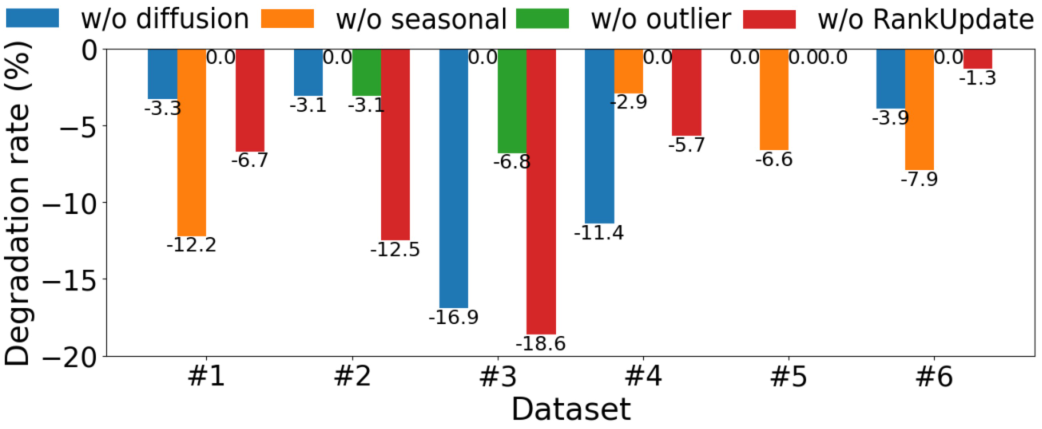
\includegraphics[width=0.95\linewidth]{figures/drop_rate.png}
  \caption{Ablation study của paper. Cột càng cao thể hiện mức giảm chất lượng khi bỏ một thành
  phần. Nguồn: Higashiguchi et al. (2025), arXiv:2505.00242v1, Figure~3; hình của tác giả,
  CC BY 4.0.}
  \label{fig:ablation}
\end{figure}

Hình~\ref{fig:ablation} bỏ lần lượt diffusion, seasonal, outlier và RankUpdate. Các degradation rate
được đo ở horizon 26 tuần (GoogleTrends) hoặc 14 ngày (Covid-19). Paper báo cáo:
\begin{itemize}
  \item seasonal cải thiện rõ ở các dataset có mùa vụ mạnh như Device, Language và Covid-19;
  \item diffusion cải thiện rõ ở VoD và Chatapp;
  \item outlier giúp ở một số dataset nhờ lọc các thay đổi đột ngột;
  \item RankUpdate giúp mô hình thích nghi khi số chiều tối ưu thay đổi.
\end{itemize}
Điều quan trọng không kém là các ngoại lệ. Ở Language, diffusion không cải thiện; paper diễn giải
rằng có thể có rất ít lan truyền giữa các quốc gia cho các ngôn ngữ lập trình. Ở dataset không có
nhiều mùa vụ/outlier, hai thành phần này có thể không giúp. Một mô hình ``thắng trung bình'' không
có nghĩa mọi module đều hữu ích ở mọi nơi.

\subsection{Q2: scalability}

\begin{figure}[htbp]
  \centering
  \begin{subfigure}[t]{0.49\linewidth}
    \centering
    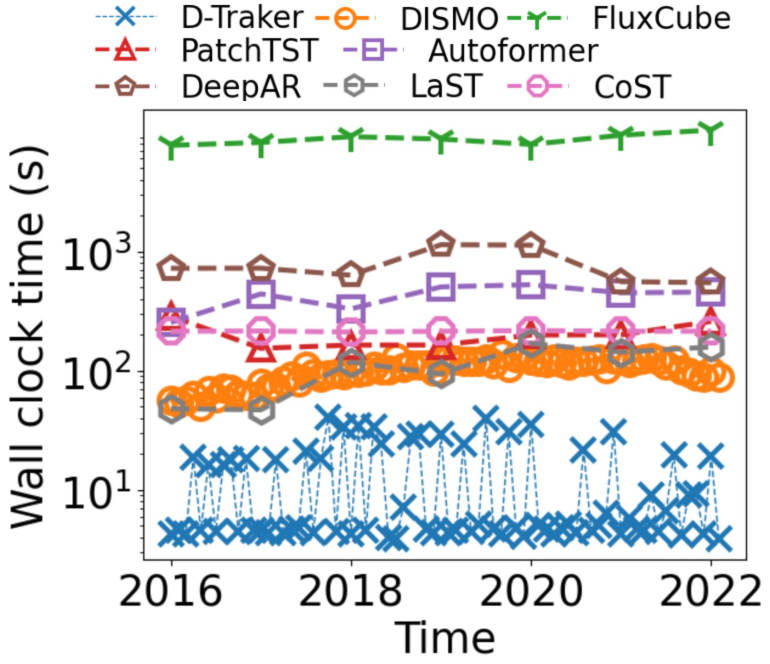
\includegraphics[width=\linewidth]{figures/scalability.png}
    \caption{Thời gian theo chiều dài stream.}
  \end{subfigure}\hfill
  \begin{subfigure}[t]{0.49\linewidth}
    \centering
    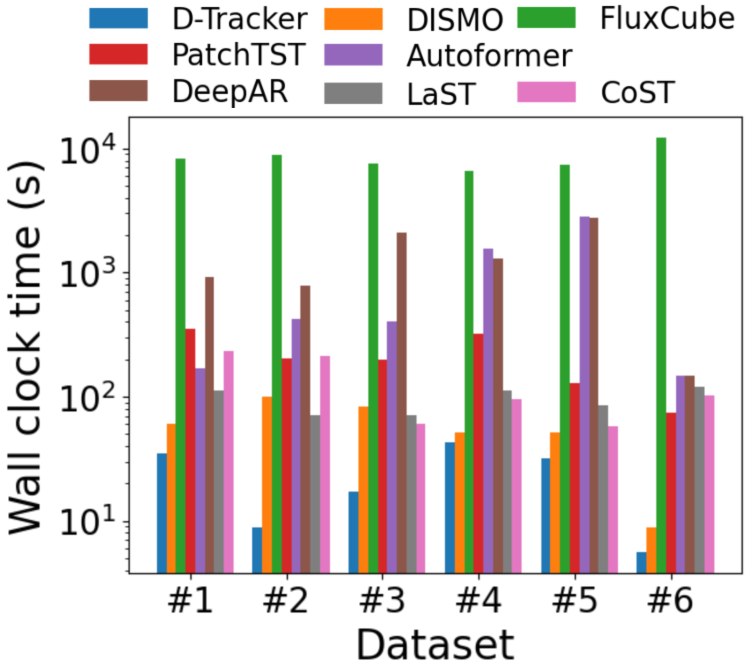
\includegraphics[width=\linewidth]{figures/avgtime.png}
    \caption{Thời gian trung bình trên toàn stream.}
  \end{subfigure}
  \caption{ Scalability của D-Tracker trên Pythonlib. Nguồn: Higashiguchi et al. (2025),
  arXiv:2505.00242v1, Figure~4; hình của tác giả, CC BY 4.0.}
  \label{fig:scalability}
\end{figure}

Ở Hình~\ref{fig:scalability}, thời gian xử lý của D-Tracker gần như phẳng khi stream dài thêm, trong
khi các baseline có xu hướng tăng. Các ``spike'' nhỏ là lúc RankUpdate chạy ModelEstimation nhiều
lần. Đây là bằng chứng cho tuyên bố ``thời gian không phụ thuộc chiều dài stream'', nhưng không
phải bằng chứng rằng mọi phép tính là hằng số: chi phí vẫn phụ thuộc số từ khóa, địa điểm, rank và
số lần cập nhật cấu trúc.

\subsection{Q3: mô hình có diễn giải được không?}

\begin{figure}[htbp]
  \centering
  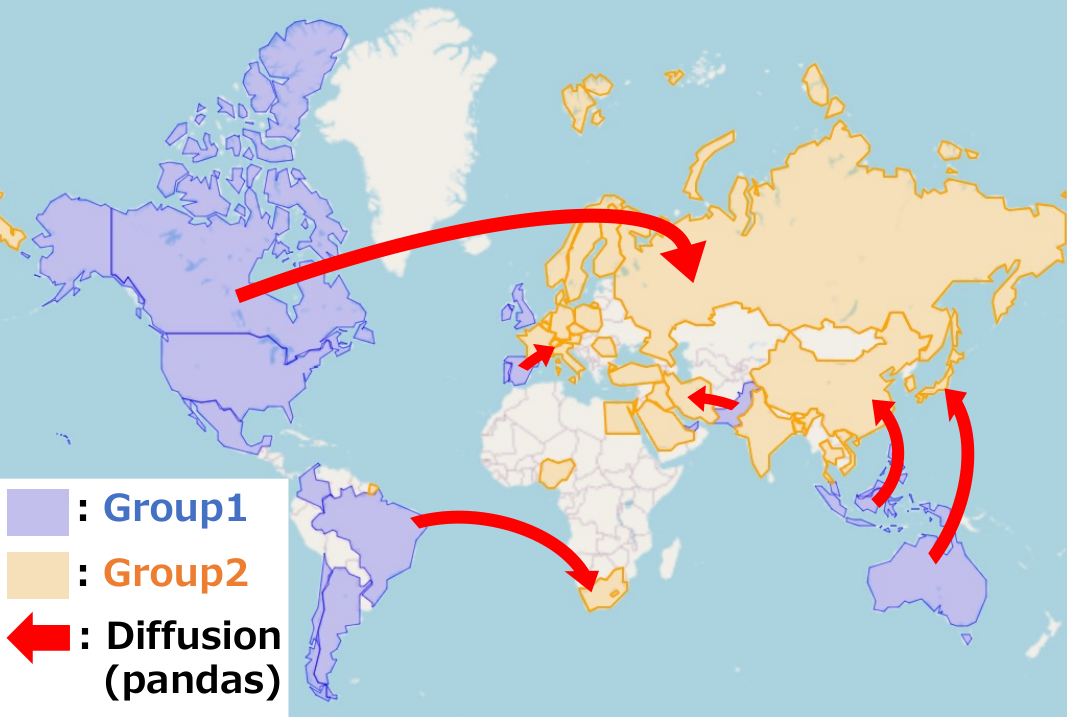
\includegraphics[width=0.78\linewidth]{figures/diff_2014.png}
  \caption{Một phần kết quả mô hình hóa Pythonlib 2013--2015: pattern lan truyền được hệ
  reaction--diffusion gán cho ``pandas''. Nguồn: Higashiguchi et al. (2025), arXiv:2505.00242v1,
  Figure~5; hình của tác giả, CC BY 4.0.}
  \label{fig:diffusion-example}
\end{figure}

Paper đọc Ví dụ~\ref{fig:diffusion-example} như sau: dynamics liên quan đến ``pandas'' lan từ nhóm
địa điểm gồm Bắc Mỹ và Australia sang nhóm gồm các nước châu Á, chủ yếu Trung Quốc. Đây là một
\emph{diễn giải có cấu trúc}: hệ số từ khóa nói ``pandas'', hệ số địa điểm chia nhóm, và tham số
diffusion nói hướng. Nó không chứng minh quan hệ nhân quả; để kiểm chứng cần dữ liệu ngoài mô hình
hoặc thiết kế thí nghiệm phù hợp.

\subsection{Điều paper không chứng minh}

Paper không báo cáo khoảng tin cậy, kiểm định thống kê hay xác suất dự báo. Nó cũng không chứng minh
D-Tracker luôn thắng mọi baseline trên mọi horizon; kết luận là trên sáu stream và các thiết lập đã
nêu. Vì vậy, câu đúng là ``trong thí nghiệm này, D-Tracker đạt MAE tốt nhất và thời gian chạy thấp
hơn'', không phải ``D-Tracker là phương pháp tốt nhất cho mọi dữ liệu chuỗi thời gian''.

\begin{keypoint}
Ba kết quả nên nhớ: (1) D-Tracker đứng đầu MAE trên sáu dataset theo paper Table~3; (2) thời gian mỗi
bước không tăng theo chiều dài stream nhờ cửa sổ cố định, với các spike khi đổi rank; (3) mô hình
cho ra các nhóm và hướng diffusion đọc được, nhưng đó là diễn giải theo giả định, không phải nhân
quả đã kiểm chứng.
\end{keypoint}

\begin{selfcheck}
\begin{enumerate}
  \item Vì sao MAE và RMSE có thể xếp hạng hai mô hình khác nhau?
  \item Trong ablation, vì sao bỏ diffusion không làm giảm chất lượng ở Language?
  \item Giải thích vì sao ``thời gian không phụ thuộc chiều dài stream'' không đồng nghĩa $O(1)$.
  \item Nêu một kết luận \emph{không} thể rút ra từ Figure~\ref{fig:diffusion-example}.
\end{enumerate}
\end{selfcheck}

\section{Đặt D-Tracker trong bối cảnh và đọc phản biện}
\label{sec:discussion}

\subsection{Related work trong một trang}

Paper chia công trình liên quan thành ba nhóm. Hiểu ba nhóm này giúp thấy D-Tracker kế thừa gì và
cố giải quyết điều gì.

\paragraph{Tensor analysis.}
Tucker, PARAFAC và PARAFAC2 là các cách phân rã tensor quen thuộc; nhiều biến thể online đã được
phát triển cho dữ liệu lớn. MLDS ghép linear dynamical system với Tucker; SMF và SSMF tập trung
vào mùa vụ và dự báo. DISMO ghép PARAFAC với phương trình vi phân phi tuyến, cho kết quả diễn giải
tốt, nhưng \emph{không} mô hình hóa lan truyền giữa các địa điểm. D-Tracker thêm đúng phần còn
thiếu đó bằng reaction--diffusion.

\paragraph{Time-series forecasting.}
Các phương pháp thống kê cổ điển gồm autoregression và Kalman filter. Họ mô hình sâu dùng CNN, RNN,
Transformer như PatchTST và Autoformer; LaST/CoST học biểu diễn trend/mùa vụ. Ưu điểm là độ chính
xác trên nhiều bài toán, nhược điểm là khó diễn giải và thường cần huấn luyện lại tốn kém, không
phù hợp trực tiếp với stream.

\paragraph{Social-activity modeling.}
Các mô hình web search từng nghiên cứu quan hệ cạnh tranh giữa từ khóa. FluxCube dùng ý tưởng
physics-informed neural network để học diffusion trong tensor, nhưng tốn thời gian vì phải ước lượng
nhóm địa điểm lặp lại. D-Tracker đặt diffusion vào một hệ phương trình nhỏ, cập nhật tăng dần.

\begin{table}[htbp]
  \centering
  \scriptsize
  \caption{So sánh khả năng theo paper Table~1. ``Có'' là đáp ứng, ``--'' là không được báo cáo
  là đáp ứng. D-Tracker là phương pháp duy nhất đáp ứng cả sáu yêu cầu theo bảng này.}
  \label{tab:capabilities}
  \begin{tabular}{@{}lccccccc@{}}
    \toprule
    & DISMO & FluxCube & PatchTST & Autoformer & DeepAR & LaST/CoST & D-Tracker \\
    \midrule
    Forecasting & Có & Có & Có & Có & Có & Có & Có \\
    Seasonality & Có & Có & -- & Có & -- & Có & Có \\
    Diffusion & -- & Có & -- & -- & -- & -- & Có \\
    Independent of length & -- & -- & -- & -- & -- & -- & Có \\
    Parameter free & Có & -- & -- & -- & -- & -- & Có \\
    Outlier & -- & -- & -- & -- & -- & -- & Có \\
    \bottomrule
  \end{tabular}
\end{table}

\subsection{Điểm mạnh thật sự}

Điểm mạnh không chỉ là ``dự báo chính xác hơn''. D-Tracker kết hợp ba thứ thường tách rời:
\begin{enumerate}
  \item một mô hình \textbf{sinh} có tham số diễn giải được (trend tăng/giảm, diffusion giữa nhóm);
  \item một cơ chế \textbf{streaming} chỉ dùng cửa sổ gần nhất;
  \item một tiêu chuẩn \textbf{MDL} để chọn cấu trúc thay vì thử tay.
\end{enumerate}
Với người làm phân tích, lợi ích là có thể nhìn một chuỗi dài và hỏi ``dynamics nào đang chi phối,
ở nhóm nào, lan theo hướng nào?'' thay vì chỉ nhận một con số dự báo.

\subsection{Giả định và giới hạn cần đọc kèm}

Đây là phần đánh giá của tài liệu, không phải các kết luận được paper chứng minh:

\begin{description}[leftmargin=1.8em,style=nextline]
  \item[Diễn giải không phải nhân quả.] Hệ reaction--diffusion là một \emph{giả định cấu trúc}. Nó
  có thể khớp một pattern trễ do yếu tố thứ ba gây ra. Paper không có thiết kế nhân quả, biến công
  cụ hay thí nghiệm can thiệp.
  \item[Phép cộng ba thành phần.] Giả định $\mathcal{X}^{c}\approx\widehat{\mathcal{X}}_d+
  \widehat{\mathcal{X}}_s+\widehat{\mathcal{X}}_o$ là mạnh. Nếu trend và mùa vụ tương tác phi tuyến,
  hoặc outlier không thưa, mô hình
  có thể phải dùng outlier quá nhiều và mất tính diễn giải.
  \item[Hệ số không âm.] Ràng buộc $\mathbf{W}\ge0$ giúp đọc nhóm và giữ dấu, nhưng cũng hạn chế
  các quan hệ cần trọng số âm (ví dụ một từ khóa làm giảm quan tâm từ khóa khác) trừ khi chúng
  được biểu diễn gián tiếp qua nhiều dynamics.
  \item[Không duy nhất.] Phân rã tensor thường không xác định duy nhất; các nhóm có thể xoay/hoán vị
  mà vẫn cho cùng tensor xấp xỉ. Vì vậy, đừng quá tập trung vào nhãn ``Group 1''; hãy đọc cấu trúc
  tương đối và kiểm tra tính ổn định.
  \item[Cửa sổ cố định.] Một cửa sổ $L_c$ cố định có thể bỏ lỡ chu kỳ dài hơn cửa sổ hoặc một sự
  kiện xảy ra trước đó. Chọn $L_c$ quá ngắn hoặc quá dài đều có hậu quả; paper dùng 104 tuần cho
  GoogleTrends và 56 ngày cho Covid-19.
  \item[Không có bất định.] Mô hình trả về điểm dự báo, không có khoảng tin cậy hay phân phối dự báo.
  Với quyết định rủi ro cao, cần bổ sung đánh giá bất định.
  \item[Dữ liệu thiếu và không đều.] Paper không trình bày cơ chế chính thức cho missing values,
  timestamp không đều hoặc thay đổi định nghĩa địa điểm. Đây là khoảng trống cần xử lý khi áp dụng.
\end{description}

\subsection{Độ tin cậy của bằng chứng thực nghiệm}

Các kết quả có điểm mạnh: sáu stream thật, bảy baseline, nhiều horizon, ablation cho từng module và
phân tích thời gian chạy. Nhưng cần đọc kèm:
\begin{itemize}
  \item không có kiểm định thống kê hay khoảng tin cậy cho chênh lệch MAE;
  \item ``tối đa 57\%'' không nêu rõ mẫu số tại chỗ, nên không thể diễn giải như một effect size
        thống nhất;
  \item tốc độ 8.0 lần gắn với phần cứng và cách huấn luyện baseline cụ thể;
  \item ablation cho thấy một số module không cải thiện ở một số dataset, đúng như paper thừa nhận;
  \item kết quả Covid-19 chỉ có hai tín hiệu (ca nhiễm, tử vong) và không đại diện cho toàn bộ động
        học dịch tễ.
\end{itemize}
Những điều này không phủ định kết quả; chúng giới hạn phạm vi kết luận.

\subsection{Khi nào nên và không nên dùng D-Tracker?}

\textbf{Nên cân nhắc} khi dữ liệu là tensor nhiều địa điểm/từ khóa theo thời gian, cần dự báo ngắn
hạn, cần gợi ý về nhóm và hướng lan truyền, và muốn cập nhật khi dữ liệu mới đến.

\textbf{Không nên dùng một mình} khi mục tiêu là suy luận nhân quả, khi dữ liệu thiếu/không đều
nghiêm trọng, khi cần khoảng tin cậy, hoặc khi số chiều quá nhỏ đến mức mô hình tensor không có lợi
thế. Trong những trường hợp đó, D-Tracker có thể là một \emph{nguồn giả thuyết} hữu ích, không phải
câu trả lời cuối cùng.

\subsection{Những câu hỏi phản biện nên chuẩn bị}

\begin{enumerate}
  \item Nếu hai vùng tăng cùng lúc do một chiến dịch toàn cầu, mô hình có luôn gán là diffusion không?
  \item Khi số regime tăng, $\mathcal{F}$ có thể lớn đến mức nào, và chi phí bộ nhớ ra sao?
  \item Các nhóm địa điểm có ổn định qua các lần chạy/khởi tạo khác nhau không?
  \item Điều gì xảy ra nếu chọn $L_c$ ngắn hơn chu kỳ mùa vụ?
  \item Vì sao dùng MDL thay vì cross-validation cho cấu trúc?
  \item Kết quả có còn đúng nếu missing values được điền theo cách khác?
\end{enumerate}
Đây là các câu hỏi hợp lệ để thảo luận, không phải lỗi chắc chắn của paper. Một số câu paper trả lời
một phần; số khác cần thực nghiệm bổ sung.

\begin{keypoint}
Giá trị của D-Tracker nằm ở \textbf{cách nó kết nối mô hình sinh, nén MDL và streaming}, không phải
ở một con số MAE đơn lẻ. Đọc paper công bằng nghĩa là vừa ghi nhận kết quả mạnh, vừa giữ rõ giả định
và giới hạn của chúng.
\end{keypoint}

\begin{selfcheck}
\begin{enumerate}
  \item Trong paper Table~1, khả năng nào chỉ D-Tracker có?
  \item Vì sao ``diffusion không cải thiện ở Language'' lại là thông tin hữu ích, không phải lỗi cần che?
  \item Nêu hai giả định có thể bị vi phạm khi áp dụng D-Tracker vào dữ liệu thực tế.
  \item Nếu cần kết luận nhân quả, cần thêm loại bằng chứng nào ngoài mô hình này?
\end{enumerate}
\end{selfcheck}


\appendix
\section{Công cụ tự học và tổng kết}
\label{app:learning}

\subsection*{D-Tracker trong một trang}

\begin{keypoint}
\textbf{Đầu vào:} cửa sổ tensor $k\times l\times L_c$ (từ khóa $\times$ địa điểm $\times$ thời gian).
\textbf{Đầu ra:} dự báo $L_f$ bước và một mô hình có thể đọc được.
\textbf{Cách làm:} tách dữ liệu thành trend + seasonal + outlier; nén trend thành lõi nhỏ; cho lõi
tiến hóa bằng reaction--diffusion; dùng ALS để ước lượng; dùng MDL để chọn số chiều, outlier và
regime; cập nhật theo cửa sổ.
\end{keypoint}

\begin{enumerate}
  \item \textbf{Vì sao khó?} Dữ liệu đa chiều, có trend/mùa vụ/diffusion/outlier, các pattern lại
        đổi theo thời gian và stream gần như vô hạn.
  \item \textbf{Vì sao tách ba thành phần?} Để không nhầm mùa vụ với trend và không để một cú sốc
        làm hỏng toàn bộ hệ số.
  \item \textbf{Vì sao nén trend?} Để biến hàng chục nghìn quan sát thành vài dynamics ẩn và hai
        bảng hệ số từ khóa/địa điểm.
  \item \textbf{Vì sao reaction--diffusion?} Để biểu diễn cả tăng trưởng cục bộ lẫn lan truyền giữa
        các nhóm địa điểm bằng tham số có ý nghĩa.
  \item \textbf{Vì sao ALS?} Vì tối ưu đồng thời mọi khối là khó; cập nhật lần lượt dễ triển khai
        hơn và giữ được các ràng buộc.
  \item \textbf{Vì sao MDL?} Để chọn độ phức tạp có căn cứ thay vì thử tay, đồng thời quyết định
        outlier và regime.
  \item \textbf{Vì sao streaming được?} Mỗi bước chỉ dùng cửa sổ $L_c$ cố định, không quét lại toàn
        bộ lịch sử.
  \item \textbf{Kết quả?} Paper báo cáo MAE tốt nhất trên sáu dataset, thời gian gần như không tăng
        theo chiều dài stream, và các nhóm diffusion đọc được; không chứng minh nhân quả.
\end{enumerate}

\subsection*{Lộ trình đọc lại paper}

\begin{center}
\small
\begin{tabular}{@{}>{\raggedright\arraybackslash}p{0.27\linewidth}>{\raggedright\arraybackslash}p{0.31\linewidth}>{\raggedright\arraybackslash}p{0.34\linewidth}@{}}
  \toprule
  Đọc gì & Mục tiêu & Tự kiểm tra \\
  \midrule
  Abstract + §1 & Nắm bài toán, ba tính chất và Figure~1 & Kể được ba thách thức bằng lời \\
  §3.1 + paper Table~2 & Hiểu ký hiệu và Problem~1 & Viết input/output bằng ký hiệu \\
  §3.2--3.3 + Eq.~(1)--(4) & Hiểu decomposition và ODE & Giải thích từng số hạng \\
  §4.1 + Eq.~(5)--(9) & Hiểu ALS, LM, multiplicative update & Nêu thứ tự cập nhật \\
  §4.2--4.3 + Eq.~(10) & Hiểu MDL và ModelUpdate & Giải thích đánh đổi fit/complexity \\
  §5 + paper Table~3 + Figure~3--5 & Đọc kết quả và ablation & Phân biệt MAE/RMSE, claim và bằng chứng \\
  Appendix A.1--A.4 & Chi tiết khởi tạo và thuật toán & Chỉ ra các chỗ paper mơ hồ \\
  \bottomrule
\end{tabular}
\end{center}

Gợi ý thời lượng cho lần đọc đầu: 20 phút cho §1--3, 35 phút cho §4, 25 phút cho §5, 20 phút cho
phụ lục. Không cần hiểu hết các phép biến đổi đại số ngay lần đầu; hãy viết lại mỗi công thức thành
một câu tiếng Việt trước.

\subsection*{Bảng ký hiệu}

\begin{longtable}{@{}>{\raggedright\arraybackslash}p{0.23\linewidth}>{\raggedright\arraybackslash}p{0.35\linewidth}>{\raggedright\arraybackslash}p{0.35\linewidth}@{}}
  \caption{Ký hiệu, kích thước và nghĩa.}\label{tab:appendix-symbols}\\
  \toprule
  Ký hiệu & Kích thước & Nghĩa \\
  \midrule
  \endfirsthead
  \toprule
  Ký hiệu & Kích thước & Nghĩa \\
  \midrule
  \endhead
  $k,l$ & số nguyên & số từ khóa, số địa điểm \\
  $t_c$ & thời điểm & thời điểm hiện tại \\
  $L_c,L_f$ & số bước & độ dài cửa sổ, tầm dự báo \\
  $\mathcal{X}^{c}$ & $k\times l\times L_c$ & tensor quan sát hiện tại \\
  $d_k,d_l$ & số nguyên & số nhóm từ khóa, địa điểm \\
  $d_s$ & số nguyên & số pattern mùa vụ \\
  $\mathcal{W}^{(\mathrm{core})}$ & $d_k\times d_l\times L_c$ & lõi trend ẩn \\
  $\mathbf{W}^{(\mathrm{key})}$ & $d_k\times k$ & hệ số từ khóa, không âm \\
  $\mathbf{W}^{(\mathrm{loc})}$ & $d_l\times l$ & hệ số địa điểm, không âm \\
  $\mathbf{A}$ & $d_k\times d_l$ & tốc độ tăng trưởng $a_{ij}$ \\
  $\mathcal{D}$ & $d_k\times d_l\times d_l$ & độ mạnh diffusion $d_{ijj'}$ \\
  $\theta$ & --- & $\{\mathbf{A},\mathcal{D}\}$ \\
  $\theta_d,\theta_s$ & --- & tham số trend, tham số mùa vụ \\
  $\Theta$ & --- & một mô hình đầy đủ \\
  $\mathcal{F}$ & --- & tập các mô hình theo regime \\
  $\widehat{\mathcal{X}}_d,\widehat{\mathcal{X}}_s,\widehat{\mathcal{X}}_o$ & $k\times l\times L_c$ & trend, seasonal, outlier \\
  $\mathbf{S}^{(\mathrm{time})}$ & $d_s\times L_c$ & pattern mùa vụ theo thời gian \\
  $\mathbf{S}^{(\mathrm{key})},\mathbf{S}^{(\mathrm{loc})}$ & $d_s\times k$, $d_s\times l$ & hệ số mùa vụ \\
  \bottomrule
\end{longtable}

\subsection*{Thuật ngữ Việt--Anh}

\begin{longtable}{@{}>{\raggedright\arraybackslash}p{0.27\linewidth}>{\raggedright\arraybackslash}p{0.33\linewidth}>{\raggedright\arraybackslash}p{0.33\linewidth}@{}}
  \caption{Thuật ngữ dùng trong tài liệu.}\label{tab:glossary}\\
  \toprule
  Tiếng Việt & English & Ghi chú ngắn \\
  \midrule
  \endfirsthead
  \toprule
  Tiếng Việt & English & Ghi chú \\
  \midrule
  \endhead
  tensor & tensor & mảng nhiều chiều \\
  luồng tensor & tensor stream & chuỗi tensor theo thời gian \\
  cửa sổ & window & phần gần nhất dùng để ước lượng \\
  tầm dự báo & forecast horizon & số bước cần dự báo \\
  phân rã tensor & tensor factorization & biểu diễn tensor bằng các nhân tố nhỏ \\
  lõi & core & tensor nhỏ chứa dynamics ẩn \\
  nhân tố/hệ số & factor & mức liên hệ của đối tượng với nhóm \\
  động học ẩn & latent dynamics & chuỗi ẩn mô tả pattern \\
  phản ứng & reaction & tăng/giảm cục bộ \\
  khuếch tán & diffusion & lan truyền giữa các nhóm \\
  mùa vụ & seasonality & pattern lặp theo chu kỳ \\
  ngoại lai & outlier & giá trị bất thường, thưa \\
  chế độ & regime & giai đoạn có cấu trúc tương đối ổn định \\
  bình phương tối thiểu xen kẽ & alternating least squares (ALS) & tối ưu từng khối \\
  mô tả ngắn nhất & minimum description length (MDL) & chọn mô hình theo tổng số bit \\
  không âm & non-negative & $\ge 0$ \\
  dự báo theo luồng & stream forecasting & dự báo khi dữ liệu đến dần \\
  độ phức tạp & computational complexity & cách chi phí tăng theo kích thước \\
  \bottomrule
\end{longtable}

\subsection*{Câu hỏi tự kiểm tra phân tầng}

\paragraph{Tầng 1 --- Nhớ và hiểu.}
\begin{enumerate}
  \item Ba thành phần của D-Tracker là gì và mỗi thành phần xử lý loại pattern nào?
  \item Vì sao $\mathbf{W}^{(\mathrm{key})}$ và $\mathbf{W}^{(\mathrm{loc})}$ phải không âm?
  \item MDL gồm hai loại chi phí nào?
  \item Vì sao chỉ dùng cửa sổ gần nhất lại giúp xử lý stream?
\end{enumerate}

\paragraph{Tầng 2 --- Áp dụng và tính toán.}
\begin{enumerate}
  \item Với $d_k=3,d_l=2,L_c=104$, lõi có bao nhiêu phần tử? Hai bảng hệ số có bao nhiêu nếu
        $k=8,l=50$?
  \item Nếu $w_{j'}=3,w_j=1,d_{jj'}=0.4,a_j=0$, đạo hàm reaction--diffusion bằng bao nhiêu?
  \item Một mô hình tăng $d_s$ từ 2 lên 3: chi phí mô hình thay đổi theo hướng nào, và vì sao
        chất lượng fit có thể tăng?
\end{enumerate}

\paragraph{Tầng 3 --- Phản biện.}
\begin{enumerate}
  \item Nêu một cơ chế ngoài diffusion có thể tạo ra pattern trễ giữa hai quốc gia.
  \item Nếu chọn cửa sổ ngắn hơn chu kỳ mùa vụ, điều gì có thể xảy ra với thành phần seasonal?
  \item Vì sao ``MAE tốt nhất'' chưa đủ để kết luận mô hình tốt cho mọi quyết định?
  \item Cần thêm thí nghiệm gì để kiểm tra các nhóm địa điểm có ổn định không?
\end{enumerate}

\subsection*{Gợi ý trả lời}

\paragraph{Tầng 1.}
(1) Trend chứa thay đổi có cấu trúc và diffusion; seasonal chứa pattern lặp; outlier chứa bất thường
thưa. (2) Để phép chiếu không đảo dấu dynamics và giữ cách đọc ``nhóm này tăng/giảm''. (3) Chi phí
mô tả mô hình và chi phí mã hóa dữ liệu dưới mô hình. (4) Chi phí mỗi bước không phụ thuộc tổng
chiều dài lịch sử, và mô hình cũ có thể được thay khi pattern đổi.

\paragraph{Tầng 2.}
(1) Lõi $3\cdot2\cdot104=624$; hệ số $3\cdot8+2\cdot50=124$. (2)
$0+0.4(3-1)=0.8$. (3) Chi phí mô hình tăng vì thêm tham số; fit có thể tốt hơn vì biểu diễn được
nhiều pattern mùa vụ hơn, nhưng chỉ giữ nếu tổng MDL giảm.

\paragraph{Tầng 3.}
(1) Một chiến dịch toàn cầu, tin tức lan nhanh, hoặc cùng chịu ảnh hưởng của một mùa/ sự kiện.
(2) Seasonal có thể bị hấp thụ sai vào trend/outlier vì mô hình không thấy đủ một chu kỳ.
(3) MAE bỏ qua bất định, chi phí, khả năng diễn giải, drift và phân bố lỗi; quyết định rủi ro cần
thêm khoảng tin cậy và kiểm định. (4) Chạy nhiều khởi tạo/seed, so sánh nhóm qua các regime, và
kiểm tra độ ổn định của hệ số hoặc dùng dữ liệu held-out theo địa điểm.

\subsection*{Checklist trước khi nói ``đã hiểu paper''}

\begin{itemize}
  \item Tôi có thể vẽ lại pipeline từ tensor đến forecast mà không nhìn tài liệu.
  \item Tôi giải thích được Eq.~(1)--(4) bằng lời, kể cả kích thước các tensor.
  \item Tôi phân biệt được $\theta$, $\theta_d$, $\Theta$, $\mathcal{F}$.
  \item Tôi nêu được vai trò của LM, multiplicative update, ALS và MDL.
  \item Tôi đọc được paper Table~3 mà không nhầm đơn vị, và không biến ``57\%'' thành một kết luận chắc chắn.
  \item Tôi nói rõ được ba điều: kết quả paper, giả định của mô hình, và giới hạn của kết luận.
\end{itemize}

\section*{\DTReferencesName}
\addcontentsline{toc}{section}{\DTReferencesName}

\small
\begin{thebibliography}{99}

\bibitem{paper}
Shingo Higashiguchi, Yasuko Matsubara, Koki Kawabata, Taichi Murayama, and Yasushi Sakurai.
\newblock D-Tracker: Modeling Interest Diffusion in Social Activity Tensor Data Streams.
\newblock In \emph{KDD '25}, 2025.
\newblock DOI: \href{https://doi.org/10.1145/3690624.3709192}{10.1145/3690624.3709192};
arXiv: \href{https://arxiv.org/abs/2505.00242}{2505.00242}.
\newblock \emph{The primary source for every equation, figure, and reported value in this guide.}

\bibitem{kolda}
Tamara G. Kolda and Brett W. Bader.
\newblock Tensor decompositions and applications.
\newblock \emph{SIAM Review}, 51(3):455--500, 2009.

\bibitem{dismo}
Koki Kawabata, Yasuko Matsubara, and Yasushi Sakurai.
\newblock Modeling Dynamic Interactions over Tensor Streams.
\newblock In \emph{Proceedings of the ACM Web Conference 2023}, 1793--1803, 2023.

\bibitem{fluxcube}
Taichi Murayama, Yasuko Matsubara, and Yasushi Sakurai.
\newblock Mining Reaction and Diffusion Dynamics in Social Activities.
\newblock In \emph{CIKM '22}, 1521--1531, 2022.

\bibitem{patchtst}
Yuqi Nie, Nam H. Nguyen, Phanwadee Sinthong, and Jayant Kalagnanam.
\newblock A Time Series Is Worth 64 Words: Long-term Forecasting with Transformers.
\newblock arXiv:2211.14730, 2022.

\bibitem{autoformer}
Haixu Wu, Jiehui Xu, Jianmin Wang, and Mingsheng Long.
\newblock Autoformer: Decomposition Transformers with Auto-Correlation for Long-Term Series Forecasting.
\newblock In \emph{Advances in Neural Information Processing Systems 34}, 22419--22430, 2021.

\bibitem{deepar}
David Salinas, Valentin Flunkert, Jan Gasthaus, and Tim Januschowski.
\newblock DeepAR: Probabilistic Forecasting with Autoregressive Recurrent Networks.
\newblock \emph{International Journal of Forecasting}, 36(3):1181--1191, 2020.

\bibitem{last}
Zhiyuan Wang, Xovee Xu, Weifeng Zhang, Goce Trajcevski, Ting Zhong, and Fan Zhou.
\newblock Learning Latent Seasonal-Trend Representations for Time Series Forecasting.
\newblock In \emph{Advances in Neural Information Processing Systems 35}, 38775--38787, 2022.

\bibitem{cost}
Gerald Woo, Chenghao Liu, Doyen Sahoo, Akshat Kumar, and Steven Hoi.
\newblock CoST: Contrastive Learning of Disentangled Seasonal-Trend Representations for Time Series Forecasting.
\newblock arXiv:2202.01575, 2022.

\bibitem{stl}
Robert B. Cleveland, William S. Cleveland, Jean E. McRae, and Irma Terpenning.
\newblock STL: A Seasonal-Trend Decomposition Procedure Based on LOESS.
\newblock \emph{Journal of Official Statistics}, 6(1):3--73, 1990.
\newblock (The paper cites this as ``STL: A seasonal-trend decomposition''.)

\bibitem{ntd}
Yong-Deok Kim and Seungjin Choi.
\newblock Nonnegative Tucker Decomposition.
\newblock In \emph{IEEE Conference on Computer Vision and Pattern Recognition}, 1--8, 2007.

\bibitem{mdl}
Jorma Rissanen.
\newblock Modeling by Shortest Data Description.
\newblock \emph{Automatica}, 14(5):465--471, 1978.

\bibitem{lm}
Jorge J. Mor\'e.
\newblock The Levenberg--Marquardt Algorithm: Implementation and Theory.
\newblock In \emph{Numerical Analysis}, Springer, 105--116, 2006.

\end{thebibliography}

\begin{keypoint}
\ifdefstring{\DTExplainerLanguage}{vi}{%
  Tài liệu này không thay thế paper gốc. Khi có khác biệt giữa bản giải thích và nguồn, paper
  arXiv:2505.00242v1 là nguồn quyết định; các điểm mơ hồ đã được nêu trong các Chương~\ref{sec:model},
  \ref{sec:mdl-streaming} và~\ref{sec:experiments}.
}{%
  This document does not replace the original paper. If the guide and the source disagree, the
  source arXiv:2505.00242v1 decides; known ambiguities are surfaced in Sections~\ref{sec:model},
  \ref{sec:mdl-streaming}, and~\ref{sec:experiments}.
}
\end{keypoint}


\end{document}
